\synctex=1
\documentclass[a4paper,11pt,svgnames]{book}

\usepackage[utf8x]{inputenc}
\usepackage{mathtools}
\usepackage{thesis}
\usepackage{calc}
\setlength{\marginparwidth}{2cm}
\setlength{\voffset}{-0.25in}
\setlength{\parskip}{0.1in}

%\usepackage{draftwatermark}
%\SetWatermarkScale{4}

\usepackage{url}

%\usepackage[spanish]{babel}
%\usepackage[T1]{fontenc}
\usepackage{tabularx}
\usepackage{graphicx}
\usepackage[usenames,dvipsnames,table]{xcolor}
\usepackage{verbatim}


\usepackage[pdftex,
    pdfauthor={Adrian Perez Orozco},
            pdftitle={Application of data mining techniques for failure prediction in a railway maintenance system},
            pdfsubject={Master Thesis},
            pdfkeywords={R, Data Mining, Sequences, Alarms, Event Prediction},
            pdfproducer={PDFTex},
            colorlinks=true,linkcolor=black,citecolor=black,urlcolor=black,hypertexnames=false]{hyperref}

%\usepackage{longtable}


\usepackage{framed}

%lstlisting
\usepackage{listings}

\lstdefinelanguage{JavaScript}{
  keywords={typeof, new, true, false, catch, function, return, null, catch, switch, var, if, in, while, do, else, case, break},
  keywordstyle=\color{blue}\bfseries,
  ndkeywords={class, export, boolean, throw, implements, import, this},
  ndkeywordstyle=\color{darkgray}\bfseries,
  identifierstyle=\color{black},
  sensitive=false,
  comment=[l]{//},
  morecomment=[s]{/*}{*/},
  commentstyle=\color{purple}\ttfamily,
  stringstyle=\color{red}\ttfamily,
  morestring=[b]',
  morestring=[b]"
}

\lstdefinestyle{mono}{
   framesep=8px,
   extendedchars=true,
   basicstyle=\ttfamily,
   showstringspaces=false,
   showspaces=false,
   tabsize=2,
   breaklines=true,
   showtabs=false,
   captionpos=b,
   xleftmargin=8pt,
   xrightmargin=8pt
}

\definecolor{chapterdetails}{HTML}{6DBAFF}

\usepackage[sf,bf]{titlesec}
\titleformat{\chapter}[display]
  {\normalfont\Large\sffamily\raggedleft}
  {\vspace{5cm}\MakeUppercase{\chaptertitlename}%
    \rlap{ \resizebox{!}{1.5cm}{\thechapter} \color{chapterdetails}\rule{5cm}{1.5cm}}}
  {10pt}{\Huge}[{\color{chapterdetails}\titlerule[0.8mm] }]
\titlespacing*{\chapter}{0pt}{30pt}{20pt}

%\titleformat{\section}{\large\sffamily\bfseries}{\thesection}{1em}{}


\newenvironment{chapterintro}
{% This is the begin code
\large\it
}
{% This is the end code
\cleardoublepage}


% Tick symbols
\newcommand{\tickYes}{\checkmark}
\newcommand{\tickNo}{\hspace{1pt}\ding{55}}
% Fancy header
\usepackage{fancyhdr}
%Fancy chapter cover style


% Fancy box
\usepackage{fancybox} 
\setlength{\fboxrule}{1 pt} \setlength{\fboxsep}{10pt} \setlength{\shadowsize}{3pt}

%Sky color definition


\begin{document}
\newcommand\litem[1]{\item{\bfseries #1 }}
\renewcommand{\arraystretch}{1.5} %Makes tables less crammed

\newcommand\headcell[1]{%
  \multicolumn{1}{|c|}{\cellcolor{DodgerBlue}\bfseries\sffamily\textcolor{white}{#1}}
}


%Cuadros por tablas
%\renewcommand{\listtablename}{Tables Index}
%\renewcommand{\tablename}{Table} 

% \renewcommand*{\lstlistingname}{List of X}

\pagenumbering{Roman}

\thispagestyle{empty}
\vspace*{3\baselineskip}
{\large{\bf PROYECTO FIN DE CARRERA}}
\vspace{0.5cm}

\begin{rm}
\begin{tabular}{p{3cm}p{10cm}}
\textbf{Título:} & Mineria de datos aplicada a la predicción de fallos en un sistema de mantenimiento ferroviario\\ 
\textbf{Título (inglés):} & Application of data mining techniques for failure prediction in a railway maintenance system\\ 
\textbf{Autor:} & Adrián Pérez Orozco \\ 
\textbf{Tutor:} & Carlos A. Iglesias Fernández\\ 
\textbf{Departamento:} & Ingeniería de Sistemas Telemáticos \\ 
\end{tabular} \end{rm} \vspace{1cm}

{\large{\bf MIEMBROS DEL TRIBUNAL CALIFICADOR}} \vspace{0.5cm}

\begin{rm}
\begin{tabular}{p{3cm}p{10cm}}
\textbf{Presidente:} & Gregorio Fernández Fernández\\
\textbf{Vocal:} & Mercedes Garijo Ayestarán\\
\textbf{Secretario:} & Carlos Ángel Iglesias Fernández\\
\textbf{Suplente:} & Marifeli Sedano Ruiz
\end{tabular}
\end{rm}
\vspace{1cm}

{\large{\bf FECHA DE LECTURA:}}
\vspace{1cm}

{\large{\bf CALIFICACIÓN:}}
\pagestyle{empty}
\cleardoublepage
\vspace*{\baselineskip}
\begin{center}
	{\LARGE\rm\textbf{UNIVERSIDAD POLITÉCNICA DE MADRID}\\
	\vspace{1.0cm}
	 ESCUELA TÉCNICA SUPERIOR DE\\ INGENIEROS DE TELECOMUNICACIÓN
	  }  \\

	 {\Large\rm Departamento de Ingeniería de Sistemas Telemáticos\\
	 Grupo de Sistemas Inteligentes  }  \\

\begin{figure}[!htbp]
	\centering
    
\includegraphics[width=0.7\textwidth]{img/logo_etsit.jpg}

\end{figure}
	\vspace{1.0cm}
	{{\LARGE\rm PROYECTO FIN DE CARRERA\\
	\vspace{1.0cm}
	 \textbf{ APPLICATION OF DATA MINING TECHNIQUES FOR FAILURE PREDICTION IN A RAILWAY MAINTENANCE SYSTEM} }}  \\
	 \vspace{1.0cm}
     \Large\rm\textbf{Adrián Pérez Orozco}\\
	 \vspace{1.0cm}
	 Marzo de 2013
\end{center}  

\cleardoublepage

\begin{tabular}{p{10cm}p{4cm}}
&\\
&\\
&\\
&\\
&\\
&\\
&\\
&\\
&\\
&\emph{Write cool quote here}\\
&\\
\end{tabular}
\cleardoublepage

\addcontentsline{toc}{chapter}{Resumen}

\begin{center}
\textbf{\large Resumen}
\end{center}

Resumen

\vfill
\textbf{Palabras clave:} key, word.


\cleardoublepage
\phantomsection
\chapter*{Abstract}
\addcontentsline{toc}{chapter}{Abstract}

The \emph{Trainmining} project, developed by the \emph{Intelligent Systems Group} along with \emph{Thales Spain}, consists on the development and implementation of a failure prediction system for a railway maintenance network, as the result of a Data Mining process.

Specifically, the project aims to provide the ability to predict future events in the railway network (corresponding to alarms and failures of diverse systems) taking as a base the events which have happened in the close past. The purpose of this task is being able to predict failure events before they happen, in order to prevent them or plan ahead for their solution in the most efficient way.

We present a general overview of Data Mining processes, as well as of some algorithms we have considered for the implementation of the system. Through these algorihtms, we can obtain predictive knowlege from databases of past events, automatically discovering relations, patterns or sequences which could allow us to predict other events with a certain confidence. Evaluation and validation processes are as well defined and described, in order to avoid overfitting and improve the overall performance of the system. After this validation process, an analysis of results is presented.

In order to demonstrate the utility of the developed system and the usefulness of the acquired knowledge, a predictive module prototype has been implemented, which generates predictions based on given input data.

Finally, alternative methods for the performed work are presented, as well as conclusions and possible future development lines.

\vfill
\textbf{Keywords:} Data mining, prediction, predictive maintenance, events, alarms, sequences, machine learning.

\cleardoublepage
%\phantomsection
\addcontentsline{toc}{chapter}{Acknowledgement}

\begin{center}
\textbf{\large Acknowledgement}
\end{center}

Acknowledgement
%\cleardoublepage
\phantomsection
\chapter*{Agradecimientos}
\addcontentsline{toc}{chapter}{Agradecimientos}

Agradecimientos
\cleardoublepage
\cleardoublepage
\tableofcontents % indice de contenidos
\addcontentsline{toc}{chapter}{Contents} % para que aparezca en el indice de 

\cleardoublepage
\addcontentsline{toc}{chapter}{List of Figures} % para que aparezca en el indice de contenidos
\listoffigures % indice de figuras

\cleardoublepage
\addcontentsline{toc}{chapter}{List of tables} % para que aparezca en el indice de contenidos
\listoftables % indice de tablas

\cleardoublepage
\cleardoublepage

%Header style
\pagestyle{fancy}
\fancyhf{}
\fancyhead[RO]{\sffamily \slshape \rightmark}
\fancyhead[LE]{\sffamily \slshape \leftmark}
%\renewcommand{\footrulewidth}{0.4pt} % grosor de la línea del pie
\fancyfoot[OR,EL]{\rmfamily \thepage} % texto derecha del pie
\pagenumbering{arabic}

\chapter{Introduction}
\begin{chapterintro}
 This chapter provides an introduction to the problem which will be aproached in this project. It provides an overview of the benefits of predictive operations in systems maintenance and how data mining techniques can be used for this purpose. Furthermore, a deeper description of the project and its environment is also given.
\end{chapterintro}
\section{Data Mining and Failure Prediction}
\label{sec:about_data_mining}Data mining is the process that results in the discovery of patterns -often unknown or unexpected- in large data sets. It gathers aspects of several fields of research, such as artificial intelligence, machine learning, statistics, and database systems. The overall goal of the data mining is to extract knowledge from an existing data set and being able to extrapolate general relations which can be lately used for prediction of patterns or future acquisitions of data. Data mining is specially interesting when it allows us to predict future events based on easy measurements that can be done over the time.

In almost every field of activity, the ability to predict events in any aspect of the environment can give a significant advantage against possible competitors, or even against possible casualties which can affect or threat the quality of the activity. It is of special interest the ability to predict failures in the production systems, as they usually entail reduction of the efficiency of the activity. Thus, preventive maintenance has become a very important activity in every large business.

Data mining can offer a simple and efficient way to perform automatised preventive maintenance. The failures can only be measured and registered once they happen, not serving for the purposes of their own prevention but probably for the prediction of future related events. Additionally, there is usually a vast amount of other data which can be easily measured and monitorised from the maintained systems, such as temperature, CPU load or network activity, for example. Data mining techniques can find relations between these easily-measurable indicators and failure happening chances, allowing the implementation of alarms or even automated procedures once they reach certain levels which indicate the imminent occurrence of a failure.

In this project, we will apply data mining techniques to a specific scenario: a maintenance system of a railway network. We will focus on preventive maintenance aids, as mentioned before, using data provided by Thales, the managing company of said maintenance system. For our project, we count on a vast amount of data for the last three years, comprising both failure logs and indicator values in several maintenance stations spread throughout Spain. This provides a perfect scenario for real data mining applications, as well as a useful output for successful prediction techniques.

\vfill

\section{Project description}
The  main goal of this project is to provide a functional prediction system for failures in the given environment: a maintenance system of a railway network.

Failure prediction is the main objective for proactive maintenance in any existing system. Developing new ways of predict when errors and failures are most likely to happen can help to prepare in advance maintenance tasks, as well as to eliminate or minimize the outage time or any other inconveniences caused by these errors.

The work described in this document corresponds to the \emph{Trainmining} project developed with Thales Spain, a company which is responsible of maintenance systems for the main railway lines in Spain. Thales has gathered large amounts of event logs throughout the last years, which will be used in this project as a source to extract information which we can later use to make predictions.
\chapter{Enabling Technologies}
\label{chap:enabling_technologies}
\section{Knowledge Discovery in Databases}
\label{sec:kdd}
The whole process we are approaching in this project is usually known as \emph{Data Mining}, or more generally, \emph{Knowledge Discovery in Databases}. A lot of research has been already done on this field which will serve as background for our project, as well as tools and algorithms which have been designed to treat similar problems and which we can adapt or use as base to develop our own\cite{chen1996data, fayyad1996kdd}.

Knowledge Discovery in Databases - or \emph{KDD} - is a term used to describe the procedure of acquiring high-level knowledge from low-level data. As a formal definition, \emph{Knowledge Discovery} is the non-trivial extraction of implicit, previously unknown, and potentially useful information from data~\cite{frawley1992knowledge}. This knowledge is usually found in the form of patterns and relations between variables which were unlikely to be related.

The KDD process involves several steps~\cite{feyyad1996data} which can be summarized as follows:

\begin{enumerate}
 \litem{Understanding the problem:} The first step involves understanding the environment we are studying and gaining relevant prior knowledge. In this step we must identify which goals we want to set for the knowledge discovery process. This is, we must identify the kind of knowledge we want to obtain and the data we can count on for this process.
 \litem{Creating a target dataset:} We will usually need to select a subset of variables from the available datasets. While the system we are studying may need a lot of variables to log events or make data relations, we will not likely need all of them to characterize our problem. Reducing the dimensionality of the problem will provide better results and ease the following steps.
 \litem{Data cleaning and preprocessing:} In this step we have to discern which data is actually relevant and significant for our study, and which is merely noise or outliers which should be disregarded. Operations such as noise modelling or mapping of missing and unknown values are also taken in this step.
 \litem{Data mining:} For this step we must first have decided the purpose of the model derived by the data mining algorithm. For example, summarization, regression, clustering and others. According to our decision, some data mining algorithms will be more appropriate than others.
 \litem{Interpretation of results:} Consists on interpreting the discovered patterns, removing those redundant or irrelevant and translating the useful ones into understandable terms.
 \litem{Consolidation of discovered knowledge:} The discovered knowledge is finally consolidated in an appropriate form. Depending on the context of our project, it might be simply documented or integrated in predictive modules for the analysed systems.
\end{enumerate}

\emph{Data Mining} comprises a large amount of different algorithms which can be used for the Knowledge Discovery process. Depending on the nature of the data on which we will apply these algorithms, and on the kind of knowledge we expect or want to acquire, we will need algorithms of different types.

Different algorithms can usually be classified in the following categories:

\begin{enumerate}
 \litem{Classification:} Learning a function that maps an item into predefined classes.
 \litem{Regression:} Learning a function that maps an item to a predicted variable.
 \litem{Segmentation:} Identifying a set of clusters to categorise the data.
 \litem{Summarization:} Finding a compact description for the data.
 \litem{Association:} Finding significant dependencies between different variables.\cite{Zhao2003association}.
 \litem{Sequence analysis:} Finding frequent sequences or episodes in data~\cite{zhao2003sequential,weiss2002predicting}.
\end{enumerate}

\subsection{Existing Algorithms}
\label{sec:algorithms}
From the previous classification, \emph{Segmentation} and \emph{summarization} algorithms seem to be obviously out of the question, as their functionality differs completely from the objectives we want to achieve in our project. \emph{Regression} algorithms are inadequate as well due to the nature of our data. We do not count on variables whose future value we want to predict.

\emph{Classification} algorithms might not seem like a good choice at first, as we do not have the need to classificate the events into any existing categories. However, if we define an appropriate set of categories and an appropriate model of items to classify, classification algorithms can be actually useful for our tasks. If we model the current events as the \emph{item} to classify, and the possible categories as the possible events which can happen in the future, we can actually classify the current situation (defined by the events which have already happened) into possible categories each defining what would happen next.

However, \emph{sequence analysis} seems to be the most appropriate category at at first glance: we count on historic data from the past and we want to find event patterns from which we can foresee future events. Patterns which are frequent offer useful information in this direction. If we know a set of several events which often happen in the same sequence, we can expect the later events in the sequence to happen once we have already seen the first ones.

These sequences offer a good starting point, but it is important to realize that \emph{frequency} in a pattern refers to the total of events happening during the observated period, and does not indicate in any way the \emph{probability} of the last events in a sequence to happen once the first ones have been acknowledged. In other words, we want to obtain predictions with a high \emph{probability} rather than a high \emph{frequency}.

In this direction, we will use the approach of the \emph{association} algorithms. Using frequent sequences as an starting point, we will build \emph{association rules} which will relate events in the form of boolean variables.

Therefore, this is the most appropriate approach, as it addresses our problem directly without the need of transforming it into a different kind of situation.

\section{The R language}
\section{The Rule Engine}
\chapter{Context and Goals definitions}
\label{chap:context_and_goals}

\section{Context Definition}
\label{sec:context}
Maintenance is one of the most important tasks to assure the quality and correct operation of any kind of system. Even the highest quality systems, built by the best engineers to operate for long periods with the least possible human assistance, will eventually be exposed to damage or malfunction. In order to avoid the negative effects that system malfunction can produce, a significant amount of resources and effort is usually needed to be put on maintenance tasks. However, putting resources and effort on maintenance procedures might still not be enough if the procedures and strategies are not adequate and efficient.

Traditionally, we have discerned between two types of maintenance procedures:
\begin{itemize}
\item \emph{Corrective maintenance} is the most common approach, although it has very important limitations. With this approach, elements of our system are repaired or replaced once they have failed or worn out, to bring them back to operation. This usually means a high downtime in operation, as no actions are taken until our system is already malfunctioning.

\item \emph{Preventive maintenance} focuses on preventing these failures. Elements can be periodically examined and analysed in order to control their operation and perform simpler procedures to adjust them before reaching malfunction and downtime. This approach means much higher costs, as a significantly bigger amount of time is needed to monitor the elements on our system and correct them. However, as downtime means business losses in almost all cases, these higher costs usually pay back in terms of loss reduction.
\end{itemize}

A balance can be easily achieved by spending on preventive maintenance not more than the losses we would suffer from downtime if we were using a corrective approach.

However, the costs of preventive maintenance can be drastically reduced by optimising procedures and using the adequate techniques. For example, we can reduce the amount of variables and magnitudes we are monitoring (and which cost us money to monitor) if we know which ones give the better insight on the status on our systems. The same can be done with corrective maintenance. If we can somehow foresee which systems are going to fail, we can be prepared and reduce impact on our business even if we cannot do anything to prevent its failure.

In both cases, \emph{prediction} can be a key element for maintenance optimisation. Either we know which are the indicators of a system deterioration which we can repair, or we know which systems are going to fail and when to be prepared and optimise corrective procedures. We can even speak of a new type of maintenance - \emph{predictive maintenance} - which embraces several techniques to try and obtain this knowledge of future events.

\section{Project Objectives}
The project \emph{Trainmining} aims to design predictive maintenance techniques on already-existing maintenance stations of a railway network. These maintenance stations monitor different elements and subsystems over a railway line and raises alarms whenever a line element fails or requires human intervention. Additionally, maintenance workers perform different preventive maintenance procedures, gathering information about several parameters on each element and performing the appropriate actions when needed. Acquisition of values and determination of necessary actions is however not automatised within the maintenance stations, and workers have to manually perform these tasks.

In order to design \emph{predictive procedures} for the railway network, we have a big amount of event logs gathered by the maintenance stations, as well as registries filled by maintenance workers when performing preventive tasks. We will therefore try to extract, from that large amount of data, knowledge on how to predict future events from current observations

In this direction, \emph{Data Mining} techniques can be extremely useful in order to find relations between patterns in environment variables and the occurrence of events, or even relations between events themselves. These relations, which may at first not be apparent for the human mind, can be obtained through different automated learning processes, and thus infer markers which will act as indicators of when and how failures can happen. In order to extract this data we will need to count on a significantly high amount of event logs, gathered during previous years, on which we will apply said techniques.

First of all, we need to define the learning objectives of our project: what kind of information we aim to extract from all the available data. In latest terms, what we want is to be able to predict future events based on events from the past. A prediction will be based on one or more past events (the \emph{antecedent}) and indicate one or more events than are likely to happen in the future (the \emph{consequent}). Furthermore, we can impose restrictions in terms of time. For instance, we should limit the temporal distance between events in the antecedent, and estimate how far in the future the consequent will happen. Finally, as giving a certain prediction that will be true \emph{everytime}, our prediction will have an associated \emph{confidence}, which can be described as the probability for our prediction to be true. A graphic representation of a generic prediction can be seen in figure~\ref{fig:ass_rule}.

Table~\ref{tab:objectives_methods} contains a summary of learning objectives, along with the working methods which will be followed for each of them as is explained in section~\ref{sec:methods}.

\begin{figure}[hbtp]
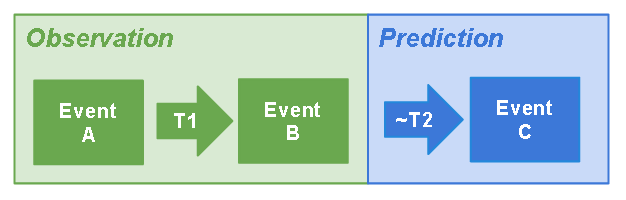
\includegraphics[width=\textwidth]{./img/association_rules.png}
\caption{A general prediction} \label{fig:ass_rule}
\end{figure}


The events forming the \emph{consequent} of our prediction will be alarms raised by the maintenance stations - we want to prevent or be prepared for the alarms happening in the future - and the antecedent can be formed by different kind of elements. In our case, both terms will be formed by system events. This means that we will predict future events taking as evidence other events which have already happened.

This working line consists of acquiring knowledge on how events are related to each other in terms of occurrence. In other terms, the events in the antecedent of our predictions will be formed by alarms (as well as the consequent, as we said before). Among all the alarms raised on the maintenance stations, some of them may be directly triggered by previous ones, having a direct occurrence relation; or might be caused by the same environmental conditions, being most likely for them to happen along the same time periods. As a result, even in cases where they might seem completely unrelated, the occurrence of one of them can give us information on the chances of others happening within a defined time span.

Our objective is to find and analyse these relations and use them to build useful predictions. Depending on the parameters we use for our knowledge discovery procedures, we might obtain different types of rules. For instance, varying the temporal resolution of our analysis, we might obtain rules to predict events in terms of months, days or hours. Depending on the timespan we work with, our prediction rules may be useful to prevent failures, to be prepared to fix them, or be completely useless if there is not enough anticipation.

It is important to note that in the railway network we are working with, there are different maintenance stations in different railway lines. Neither the maintenance stations or the lines are equal throughout the whole network, and therefore we may have to follow different procedures and expect different results for each of them. Initially, we will treat every station (along with the set of elements under its management) independently, even though we already know their classification and the similarities between them. Unless generalisation is evident and clearly convenient, we will always maintain this separation and obtain a different set of rules for each of them.

Due to the characteristics and large size of the available data, we are likely to find a vast amount of frequent sequences and association rules from which not all of them will be useful for maintenance purposes. Different metrics can be applied to evaluate the \emph{importance} of a rule, such as its confidence (its probability to be true on a given situation), the severity of the predicted events, or its support (absolute frequency of the sequence happening).

A comprehensive analysis is necessary to extract the most useful association rules from the set and discard the others, in order to obtain the most efficient set possible. Additionally, the different metrics can even allow predictions to be filtered in real time, according to the available resources or the desired results.

In figure~\ref{fig:demo_view} we can view an example use case. A maintenance operator could view the alarms which are being raised by the maintenance station (in a similar way as the current systems) and a list of predicted alarms - along with the confidence of the prediction and an estimated time span - based on those past and current alarms.

\begin{figure}[hbtp]
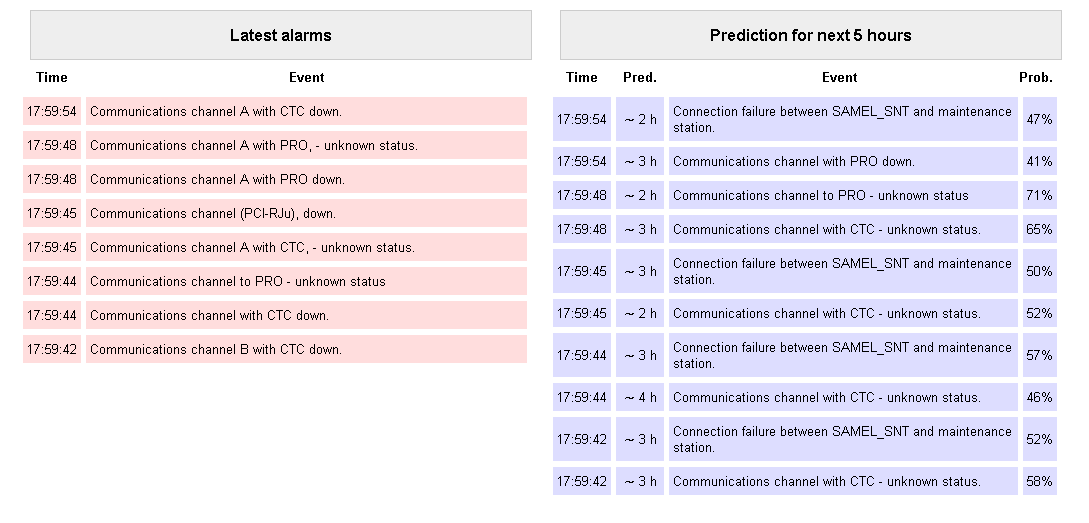
\includegraphics[width=\textwidth]{img/demo_thales.png}
\caption{An example use case} \label{fig:demo_view}
\end{figure}

\section{Data Description}
For this project, Thales Group, a leader company in the development of railway systems in Spain is cooperating with the research group {\it Grupo de Sistemas Inteligentes} from the Universidad Politécnica de Madrid, with large expertise in the application of intelligent systems to real problems. Thales Spain has developed an advanced system called \emph{maintenance station}, which diagnoses, gathers and visualises different kind of events happening along the railway network. These maintenance stations comprise different advanced diagnosis systems, which can identify and report several kind of events happening along the lines which might require human intervention. These stations gather logs with all the events which have happened in the past, which will allow us to study and analyse the operation of these stations during the past.

At the moment of writing this document, we count on data of four maintenance stations (A, B, C and D), which are located in Spain. Each of these stations controls a different railway line, and have different diagnosis systems and characteristics, as shown in table~\ref{tab:stations}. In this table we see that the three lines we are working with are of different types and have different diagnosis systems. Specifically, Stations A, B and C control high speed lines, while Station D controls a commuter line. Different types of lines will have different elements and systems, and results are therefore expected to be different in both groups. Furthermore, supervised systems are different in all the three stations, which means that alarms received from each of them will not necessarily be the same. Details on number of events and time span of the available data is given on table~\ref{tab:data_details}.

\begin{table}
\begin{center}
\begin{tabular}{|c|c|c|}
\hline \headcell{Name} & \headcell{Line type} & \headcell{Supervised systems} \\ 
\hline
\hline Station A & High Speed & SAM-E-L \\
\hline Station B & High Speed & SAM-E-L \\ 
\hline Station C & High Speed & ERTMS (levels 1 and 2) \\ 
\hline Station D & Commuter & Diagnosis and Energy \\ 
\hline 
\end{tabular}
\\
\bigskip
ERMTS: European Rail Traffic Management System\\
SAM-E-L: Sistema de Ayuda al Mantenimiento para Ence (Local)\\

\end{center} 
\caption {List of studied maintenance Stations} \label{tab:stations} 
\end{table}

\begin{table}
\begin{center}
\begin{tabular}{|c|c|c|c|c|}
\hline \headcell{Station} & \headcell{Events} & \headcell{Dates} & \headcell{Period} \\ 
\hline
\hline Station A & 545774 & 02/12/2010 - 03/10/2012 & 2 years \\
\hline Station B & 239470 & \begin{tabular}[C]{@{}c@{}}18/01/2010 - 31/05/2010\\10/02/2012 - 20/07/2012\end{tabular}  &  10 months \\ 
\hline Station C & 304408 & 30-11-2007 to 03-06-2009 &  1.5 years \\ 
\hline Station D & 118026 & 17-05-2011 to 09-04-2012 &  1 year \\ 
\hline 
\end{tabular}
\end{center} 
\caption {Summary of available data} \label{tab:data_details} 
\end{table}

\subsection{Database description}
\label{sec:database_description}
In order to properly process the data provided in form of database backups, it is of essential importance that we completely understand how data is represented in databases. We will analyse the structure and how data is represented in the provided databases (one for each station). Each of these databases corresponds to a single \emph{maintenance station}, which comprises a whole railway line with several elements along it. The elements with diagnosis systems which can raise alarms are called \emph{installations}, and have different sets of sensors and other systems to control \emph{field elements}. An schematic representation of this architecture is represented in figure~\ref{fig:arch_stations}. The detailed description of available systems and subsystems is of few interest to us. Initially we will only need to differentiate between maintenance stations and installations.

\begin{figure}[hbt]
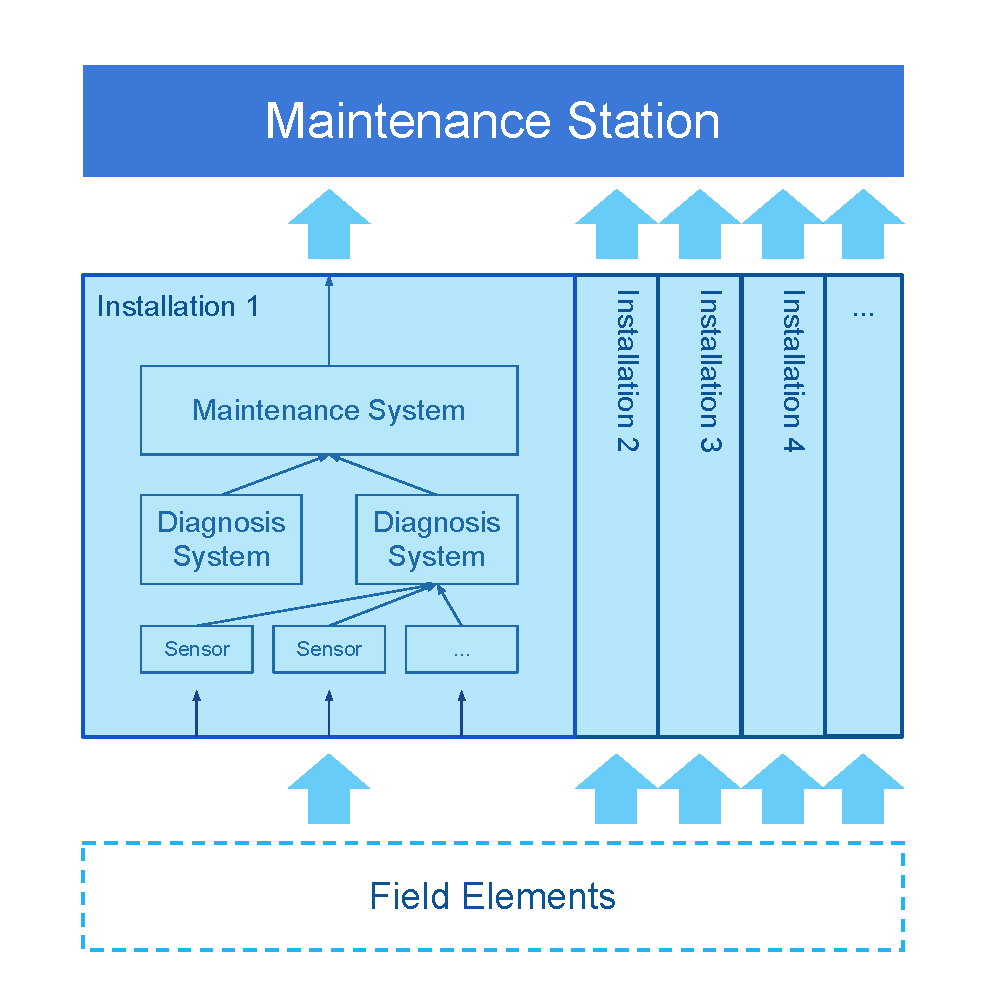
\includegraphics[width=\textwidth]{./img/arch_stations.pdf}
\caption{Simplified diagram of the maintenance systems architecture} \label{fig:arch_stations}
\end{figure}

Each \emph{maintenance station} has its own unique database, which is of great convenience in order to treat different stations independently. We will start analysing the structure of the main tables of said databases. Due to the high complexity of the maintenance stations, there are a vast amount of tables with configuration parameters and other operational values which are not of interest for our purposes. With assistance from Thales engineers, we have reduced the tables only to those which characterise registered alarms. A total of three different tables are used in order to register this information, which are the following:

\begin{description}
\item[ALARMS table] This table contains an entry for every alarm received by the maintenance station. Its fields are detailed on table~\ref{tab:table_er_errors}.
\item[INSTALLATIONS table] This table contains information on all the installations managed by the maintenance station. Its fields are detailed on table~\ref{tab:table_ig_installationgeneral}
\item[ALARM\_DETAILS table] This table contains detailed information about the alarms. Its fields are detailed on table~\ref{tab:table_ers_errors_sam_ence}
\end{description}

Concluding, for each alarm we will have a timestamp and an alarm identifier in table ALARMS. Alarm identifier is a foreign key which points to table ALARM\_DETAILS in which further details of the alarm are saved. Among these details, we can find an installation identifier which specifies which installation has produced the alarm. That identifier is also a foreign key pointing to table INSTALLATIONS, in which further details about the installation are stored. Further details on all the database fields are given in tables~\ref{tab:table_er_errors}, \ref{tab:table_ig_installationgeneral} and \ref{tab:table_ers_errors_sam_ence}.


\begin{table}
\begin{tabularx}{\textwidth}{|l|X|}
 \hline \headcell{Field name} & \headcell{Description} \\
 \hline
 \hline ERRORNUMBER & Alarm identifier \\
 \hline ERRORTIME & Time-stamp for the alarm \\
 \hline INSTALLATIONCODE & Code of the installation in which the alarm was raised \\
 \hline
\end{tabularx}
\caption{Detail of fields on table ALARMS} \label{tab:table_er_errors}
\end{table}

\begin{table}
\begin{tabularx}{\textwidth}{|l|X|}
 \hline \headcell{Field name} & \headcell{Description} \\
 \hline
 \hline INSTALLATIONCODE & Installation identifier  \\
 \hline SHORTNAME & Short name of the installation \\
 \hline LOCATION & Location for the installation \\
 \hline
\end{tabularx}
\caption{Detail of relevant fields on table INSTALLATIONS} \label{tab:table_ig_installationgeneral}
\end{table}

\begin{table}
\begin{tabularx}{\textwidth}{|l|X|}
 \hline \headcell{Field name} & \headcell{Description} \\
 \hline
 \hline ERRORNUMBER & Alarm identifier \\
 \hline EVENT\_TYPE & Defines the type of alarm which has been generated. Its possible values are listed in table~\ref{tab:field_event_type}. \\
 \hline ADDITIONAL\_TEXT & Alarm code \\
 \hline ADDITIONAL\_INFOS & Additional parameters to be shown in error message \\
 \hline ERRORCATEGORY & Alarm severity. Values from 1 to 5 indicating importance of the alarm, or -1 if the alarm indicates recovery from a previous failure. \\
 \hline
\end{tabularx}
\caption{Detail of fields on table ALARM\_DETAILS} \label{tab:table_ers_errors_sam_ence}
\end{table}

\begin{table}
\begin{tabularx}{\textwidth}{|l|X|}
  \hline \headcell{Event type} & \headcell{Description} \\
  \hline
  \hline fieldElementAlarm & Alarm related to a field element \\
  \hline fieldElementFailure & Failure in a field element \\
  \hline operatorInformation & Information to the operator \\
  \hline imCpuAndCommunications & Related to IM CPU or IM communications \\
  \hline internalDiagnosis & Internal diagnosis of a system \\
  \hline operationsDiagnosisCommunications & Communication error in Operation and Diagnosis systems \\
  \hline ImFecVersions & IM or FEC version \\
  \hline internalTraces & Internal traces of a system \\
  \hline operatorCommandAnswer & Answer to an operator command \\
  \hline CommProblem & Undefined communication problem \\
  \hline Information & Information message: versions, etc. \\
  \hline CommunicationsAlarm & Procedures and processes to carry information from one point to other \\
  \hline QualityOfServiceAlarm & Loss of quality of service \\
  \hline ProcessingErrorAlarm & SW or processing error \\
  \hline EquipmentAlarm & Equipment failure \\
  \hline EnvironmentAlarm & Related to the environment where the system is located \\
  \hline other & Other \\
  \hline
\end{tabularx}
\caption{Description of values for the field EVENT\_TYPE} \label{tab:field_event_type}
\end{table}
\clearpage

\subsubsection{Reduced representation of alarms}
\label{sec:reduced_alarms}
In section~\ref{sec:database_description} we have seen a deep definition of all the tables characterising registered alarms. Each of these tables contain several fields, which in total makes an inconvenient large number of variables. While all of them are necessary for correct system function and maintenance purposes, not all of them will be necessary for us to work with alarms.

In order to characterise an event, the main things we need to know can be reduced to three variables:
\begin{itemize}
\item What has happened
\item When has it happened
\item Where has it happened
\end{itemize}

In section~\ref{sec:database_description} we have seen other variables which can provide additional information which - although not essential - can be useful. Specifically, we think the following data can be of possible interest:

\begin{itemize}
\item How severe the event is (severity)
\item Which type of event has happened (event type)
\end{itemize}

These variables can help us to classify alarms or give more importance to those which are more severe. As this information is already provided on given databases, we will keep it and use it for better alarm classification and filtering. However, none of them are essential in order to characterise alarms, as both of them give information which is already implicit in our previous \emph{``what has happened''} variable. Specifically, this information will be of great help in order to make a preliminary statistical insight on the events of the databases, for which a generalisation in terms of severity and category can help us have a better overview of the situation.

We have to identify which fields on our database corresponds to each of the variables we want to obtain. A direct relation is not possible, as details on \emph{what} has happened is registered in several fields of the database. This is necessary for maintenance purposes and better alarm handling in the maintenance station, but for our purposes we should identify \emph{what} has happened with a single variable.

In our database, we have unique alarm identifiers for each of the alarms. For better handling and understanding of what is happening, we will use the textual identifier of the events to identify them. This identifier is gathered on the \emph{ADDITIONAL\_TEXT} field, and can be translated to a full comprehensive human-readable message by the maintenance station. Furthermore, there is additional data to fill in details about the message. For example, we can have an alarm such as ``Communication channel with \emph{X} down'', being \emph{X} an additional parameter saved in the \emph{ADDITIONAL\_INFOS} field. Here we can follow two different approaches: disregard the information about \emph{X}, and just treat it as a ``Channel down'' error; or easily build a compact representation including both variables, such as ``channel.down/x''.

\subsection{Data preprocessing}
As we already mentioned, most data mining processes are usually focused on predicting the value of some variables given the value of the rest variables in a given observation. They work with discrete observations for which each of the variables is analysed or predicted. In our databases we have continuous observations, which need to be transformed into discrete observations\cite{zaki2001spade}.

Depending on the specific application we are using, we can need to transform this data into two possible formats. The first one is the called \emph{basket format}. The most typical example usually used to explain it is a registry of clients of a shop which keeps lists of what the clients buy (hence the name). Therefore, for each observation (often called \emph{transactions} again as an analogy to clients buying in a shop) we will have a list of items happening during that observation (or bought in that transaction). It is important to note that we will keep the same number of variables as in our original data, only that we will stack several items in single entries to obtain discrete observations. It is also important to be careful with which variables we are stacking. While we need to combine all the alarms happening during the same period, it is important not to lose or combine the Installation value. As a result, time identifiers won't be unique in the whole transformed database, but the pair time 
identifier-installation identifier will.

An example can be seen in tables \ref{tab:data_before_discret} and \ref{tab:basket_example}. Table~\ref{tab:data_before_discret} is an example of the original data, and table~\ref{tab:basket_example} is the equivalent data transformed into basket format.

The second possible transformation is to represent the occurrence of each alarm with an additional variable. This means that we will need as many variables as the total number of possible different alarms in our system. Same as before, we must be careful to preserve data on installations, and create independent observations for each time slot and each installation. Each additional variable can represent the alarms in different ways. Either in a boolean sense (whether the alarms happens at least once or not at all) or the specific number of times the alarm has happened. In order not to lose information at this stage of processing, we will keep the specific amount of times each alarm has happened, which can be easily reduced to a boolean variable if appropriate for the application.

This second case is indeed a more strict representation of the \emph{basket format}. While in basket format we just needed a single variable where we could add all the alarms in the form of a list, here we need to specify exactly the number of times all the variables have happened. Both of them are equivalent and we can easily convert data from one format to another, but as different algorithms will work specifically with one of each forms of representation, it's convenient to perform both transformations from original data and use each one accordingly.

An example of this transformation can be seen in tables \ref{tab:data_before_discret} and \ref{tab:expanded_example}. Table~\ref{tab:data_before_discret} is an example of the original data, and table~\ref{tab:expanded_example} is the equivalent data discretised with additional variables.

These transformations have been automatised with R scripts, in a way so we can easily repeat these processes for different time spans. This will allow us to work at any moment with different time resolutions without any significant additional work for further transformations.

\begin{table}
\begin{center}
\begin{tabular}{|c|c|c|}
\hline \headcell{Timestamp} & \headcell{Installation} & \headcell{Alarm} \\ 
\hline
\hline 01-01-2011 00:00 & 0 & Alarm A \\ 
\hline 01-01-2011 00:30 & 0 & Alarm B \\ 
\hline 01-01-2011 00:45 & 1 & Alarm B \\ 
\hline 01-01-2011 01:10 & 0 & Alarm C \\ 
\hline 01-01-2011 01:20 & 0 & Alarm A \\ 
\hline 01-01-2011 01:22 & 0 & Alarm A \\
\hline 01-01-2011 01:25 & 1 & Alarm C \\ 
\hline 01-01-2011 01:30 & 1 & Alarm A \\ 
\hline 01-01-2011 02:20 & 0 & Alarm A \\ 
\hline 01-01-2011 02:30 & 1 & Alarm A \\ 
\hline 01-01-2011 02:45 & 0 & Alarm B \\ 
\hline ... & ... & ... \\ 
\hline 
\end{tabular} 
\end{center} 
\caption {Continuous observation. Example of alarms in log format.} \label{tab:data_before_discret} 
\end{table}

\begin{table}
\begin{center}
\begin{tabular}{|c|c|c|}
\hline \headcell{Time} & \headcell{Installation} & \headcell{Alarms} \\ 
\hline
\hline 0 & 0 & A, B \\ 
\hline 0 & 1 & B \\ 
\hline 1 & 0 & C, A, A \\ 
\hline 1 & 1 & C, A \\ 
\hline 2 & 0 & A, B \\ 
\hline 2 & 1 & A \\ 
\hline ... & ... & ... \\ 
\hline 
\end{tabular} 
\end{center}
\caption{An example of discretised data in basket format.} \label{tab:basket_example}
\end{table}

\begin{table}
\begin{center}
\begin{tabular}{|c|c|c|c|c|}
\hline \headcell{Time} & \headcell{Installation} & \headcell{Alarm A} & \headcell{Alarm B} & \headcell{Alarm C} \\ 
\hline 
\hline 0 & 0 & 1 & 1 & 0 \\ 
\hline 0 & 1 & 0 & 1 & 0 \\ 
\hline 1 & 0 & 2 & 0 & 1 \\ 
\hline 1 & 1 & 1 & 0 & 1 \\ 
\hline 2 & 0 & 1 & 1 & 0 \\ 
\hline 2 & 1 & 1 & 0 & 0 \\ 
\hline ... & ... & ... & ... & ... \\ 
\hline 
\end{tabular} 
\end{center} 
\caption {Example of discretised data} \label{tab:expanded_example} 
\end{table}

\clearpage


\section{Data Analysis}
In order to obtain a first general insight of what has happened during the time comprised by our backup data, we will perform a high-level preliminary statistic analysis. In order to achieve a qualitative idea of the type of events, we will use the additional variables we mentioned in section~\ref{sec:reduced_alarms}: severity and event type. These variables provide an already given alarm classification of interest for maintenance operators.

For this purpose, the R language provides a large amount of useful tools which can handle large amounts of data in a very efficient way\cite{quick2010statistical}.

\subsection{Event type distribution}
The first analysis we will perform consists on checking which event types appear in each maintenance station, and which percentage of the total amount of alarms corresponds to each of them. This will help us understand the nature of the events which are usually happening on our railway line.

First of all we will obtain a list of all the types found in each of the stations. We already described in table~\ref{tab:field_event_type} all the possible values for this field, but depending on the diagnosis systems installed on each of the stations, a different subset of them will be used. The list of events for each of the stations is given in tables \ref{tab:field_event_type_antequera} (Stations A, B and D) and \ref{tab:field_event_type_segovia} (Station C).

\begin{table}
\begin{tabularx}{\textwidth}{|l|X|}
  \hline \headcell{Event type} & \headcell{Description} \\
  \hline
  \hline fieldElementAlarm & Alarm related to a field element \\
  \hline fieldElementFailure & Failure in a field element \\
  \hline operatorInformation & Information to the operator \\
  \hline imCpuAndCommunications & Related to IM CPU or IM communications \\
  \hline internalDiagnosis & Internal diagnosis of a system \\
  \hline operationsDiagnosisCommunications & Communication error in Operation and Diagnosis systems \\
  \hline CommunicationsAlarm & Procedures and processes to carry information from one point to other \\
  \hline
\end{tabularx}
\caption{Event types found in Stations A, B and D} \label{tab:field_event_type_antequera}
\end{table}


\begin{table}
\begin{tabularx}{\textwidth}{|l|X|}
  \hline \headcell{Event type} & \headcell{Description} \\
  \hline
  \hline CommProblem & Undefined communication problem \\
  \hline Information & Information message: versions, etc. \\
  \hline CommunicationsAlarm & Procedures and processes to carry information from one point to other \\
  \hline ProcessingErrorAlarm & SW or processing error \\
  \hline EquipmentAlarm & Equipment failure \\
  \hline EnvironmentAlarm & Related to the environment where the system is located \\
  \hline
\end{tabularx}
\caption{Event types found in Station C} \label{tab:field_event_type_segovia}
\end{table}

From these tables we can observe that alarm types in Stations A, B and D are the same. From this we can infer that diagnosis systems in these two stations are the same or very similar, as confirmed by Thales' engineers. Station C however presents a different - although also expectedly similar - set of alarm categories. This is an indicator of diagnosis systems being very different in Station C than in the other two stations, as confirmed by Thales' engineers.

For better overview of distribution of these alarm types, we will create charts of their respective percentages for each of the stations. These charts can be seen in figures \ref{fig:albacete_chart} (Station A), \ref{fig:antequera_chart} (Station B), \ref{fig:segovia_chart} (Station C) and \ref{fig:sevilla_chart} (Station D).

\begin{figure}[htb]
 \centering
 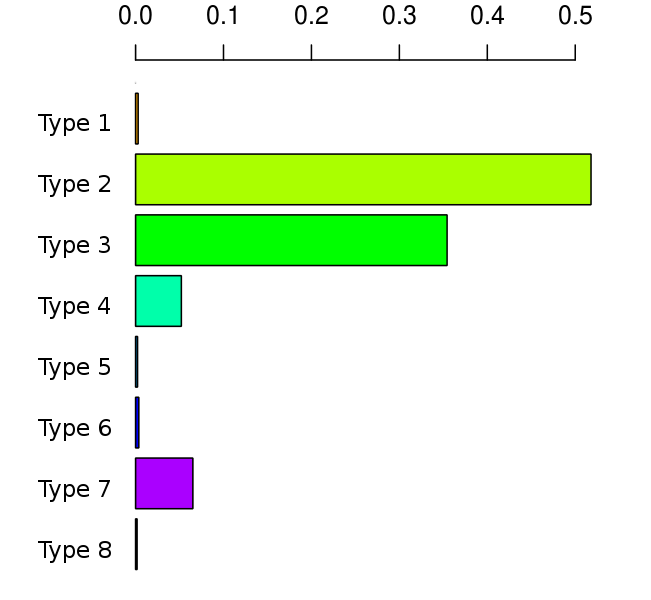
\includegraphics[width=\textwidth]{./img/albacete_graph.png}
 \caption{Alarm information for Station A}
 \label{fig:albacete_chart}
\end{figure}
\begin{figure}[htb]
 \centering
 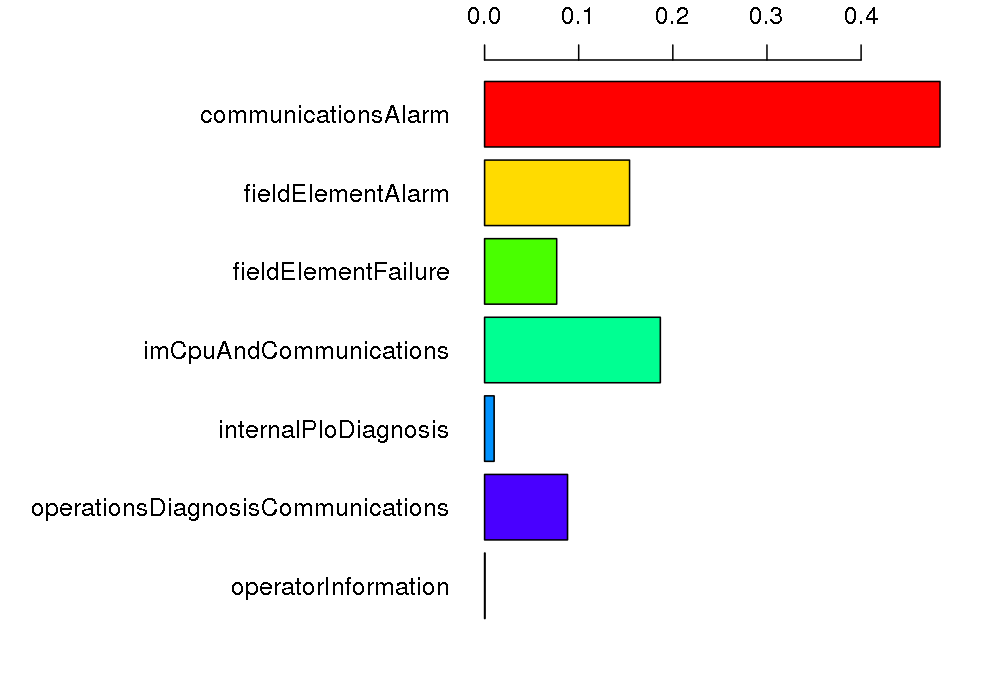
\includegraphics[width=\textwidth]{./img/antequera_graph.png}
 \caption{Alarm information for Station B}
 \label{fig:antequera_chart}
\end{figure}
\begin{figure}[htb]
 \centering
 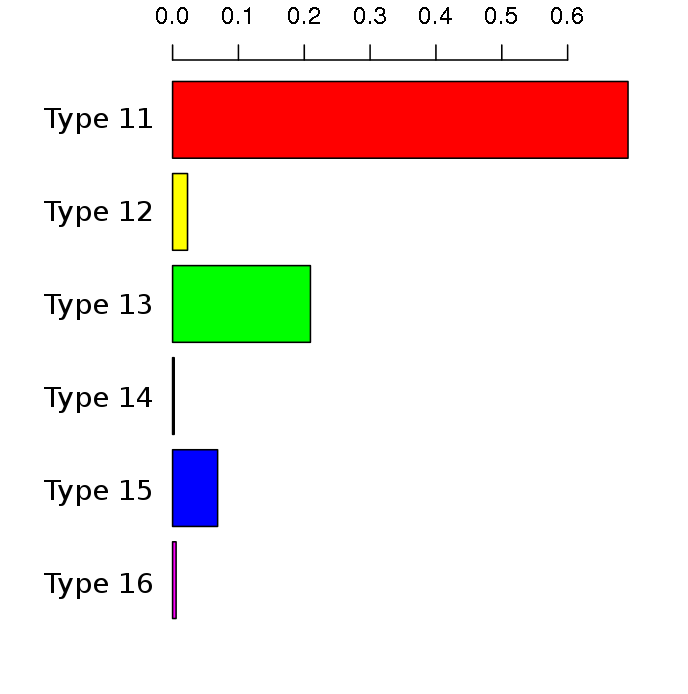
\includegraphics[width=\textwidth]{./img/segovia_graph.png}
 \caption{Alarm information for Station C}
 \label{fig:segovia_chart}
\end{figure}
\begin{figure}[htb]
 \centering
 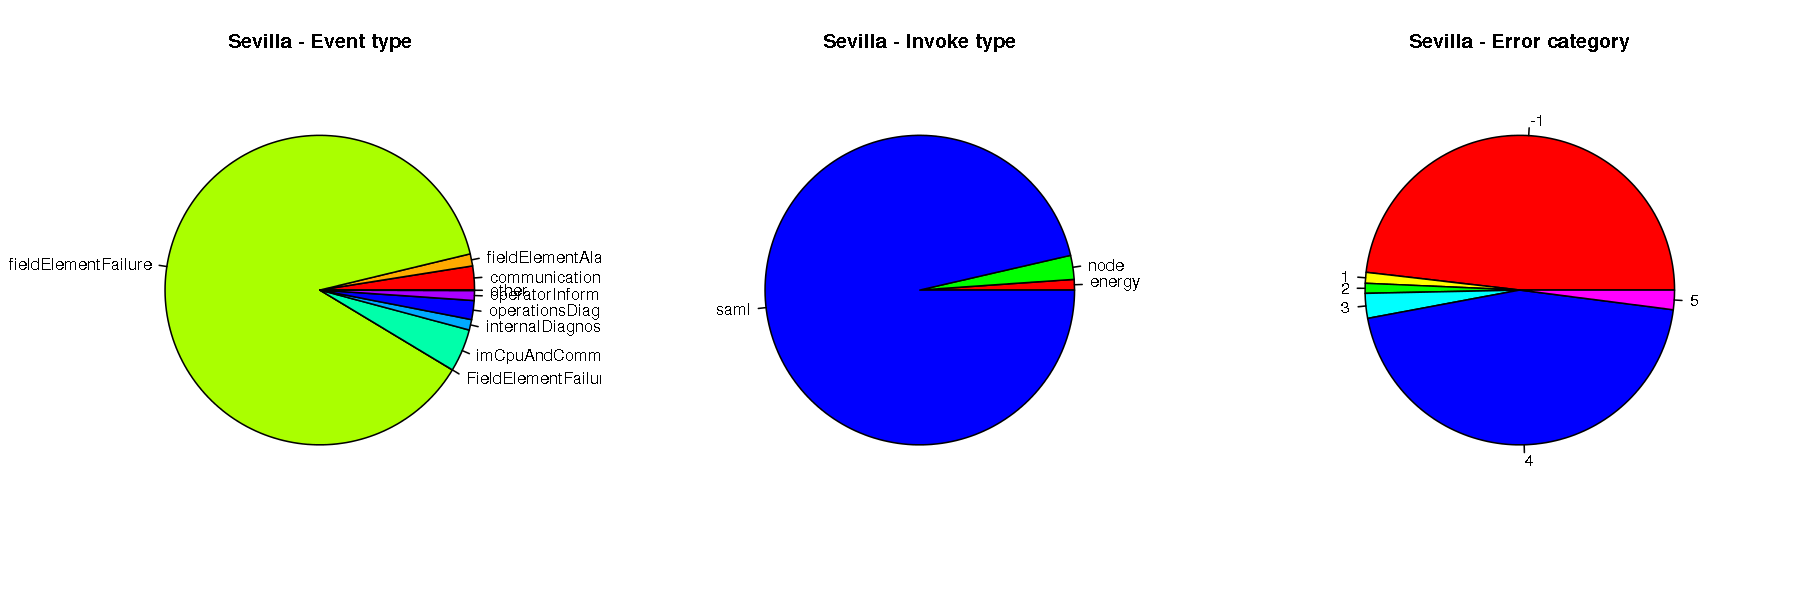
\includegraphics[width=\textwidth]{./img/sevilla_graph.png}
 \caption{Alarm information for Station D}
 \label{fig:sevilla_chart}
\end{figure}

\clearpage

We can see that in all of the stations, a single alarm type predominates among all of them. Specifically, we have a vast majority of communication alarms in Stations B and C, and a majority of field element failure alarms in Stations A and D. This is not surprising due to the considerable differences between all of them, but can become a problem as the other categories may be too small compared to these main ones when performing Data Mining techniques, obtaining less information - or none at all - from them.

In this direction, it is possible that further actions are required in order to compensate these differences, and avoid that more frequent alarms overshadow the less frequent ones.

\subsection{Daily correlation}
In order to find further differences or similarities between the different stations, we will observe how alarm types are correlated to each others\cite{edwards1976introduction}. That is, how frequent is to find alarms of two specific types happening together during the same short period. For a first insight, we will analyse correlation during daily observations. This correlation information will not be of immediate help in order to predict alarms, as predicting the most frequent alarm type given some conditions is of very little - if any - help. However, it will give us a first idea on how strongly alarms are related to each others.

The result of this correlation is represented in figures \ref{fig:albacete_corr} (Station A), \ref{fig:anteq_corr} (Station B), \ref{fig:segovia_corr} (Station C) and \ref{fig:sevilla_corr} (Station D).

\begin{figure}[htb]
 \centering
 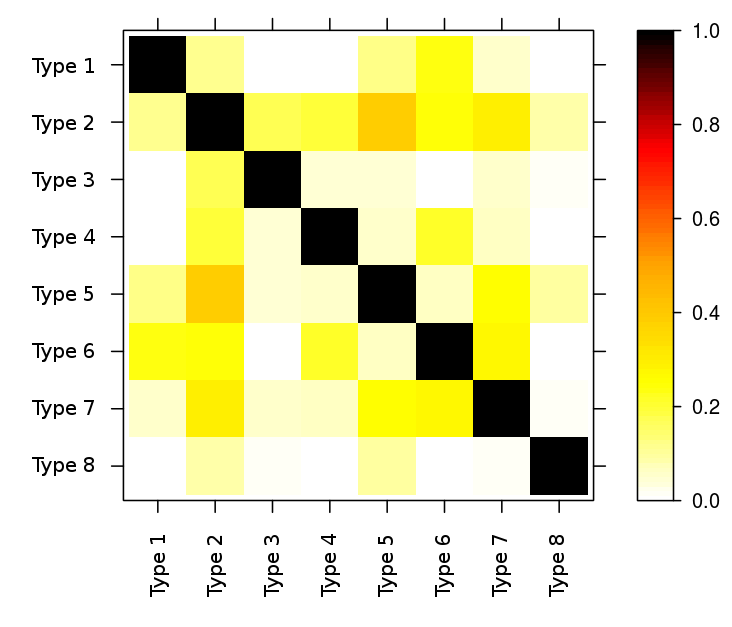
\includegraphics[width=\textwidth]{./img/albacete_corr.png}
 \caption{Daily correlation for Station A} \label{fig:albacete_corr}
\end{figure}
\begin{figure}[htb]
 \centering
 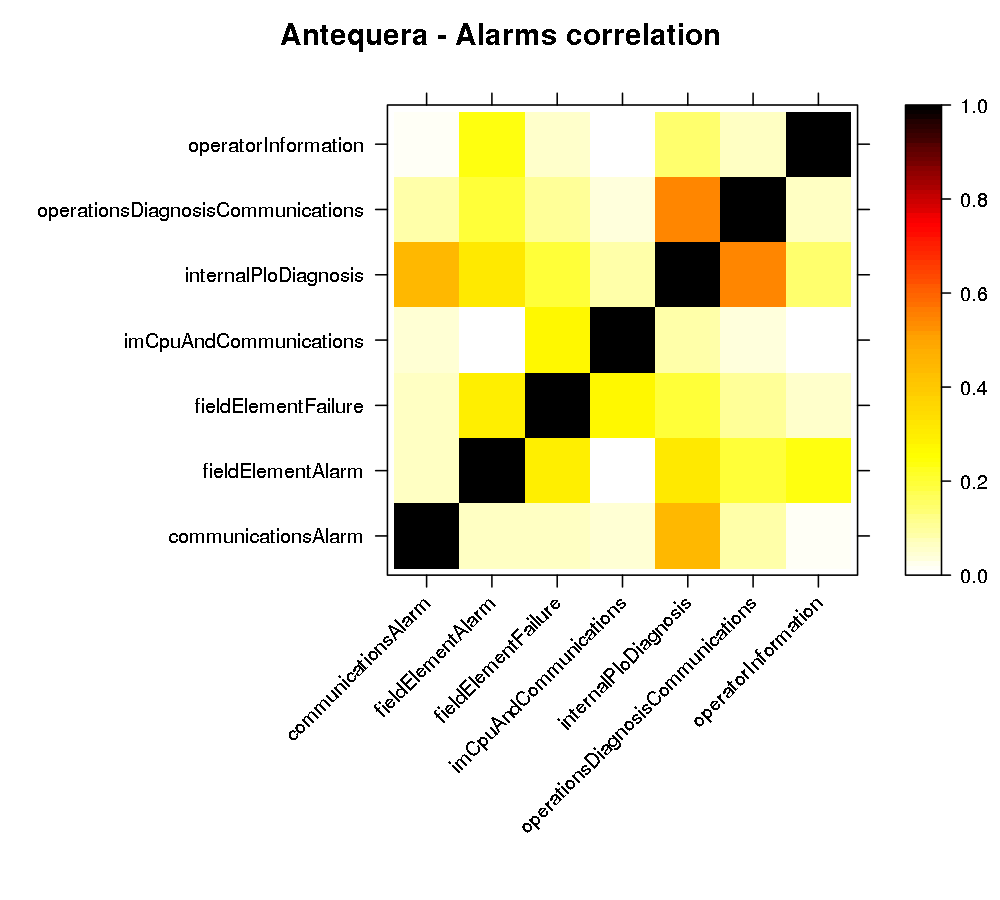
\includegraphics[width=\textwidth]{./img/antequera_corr.png}
 \caption{Daily correlation for Station B} \label{fig:anteq_corr}
\end{figure}
\begin{figure}[htb]
 \centering
 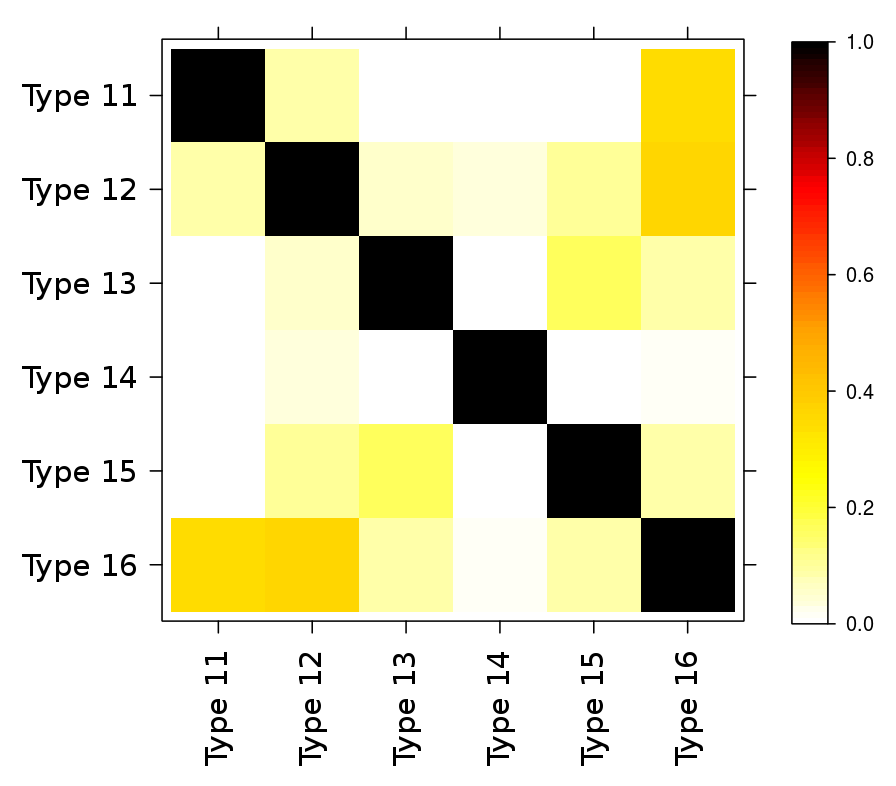
\includegraphics[width=\textwidth]{./img/segovia_corr.png}
 \caption{Daily correlation for Station C} \label{fig:segovia_corr}
\end{figure}
\begin{figure}[htb]
 \centering
 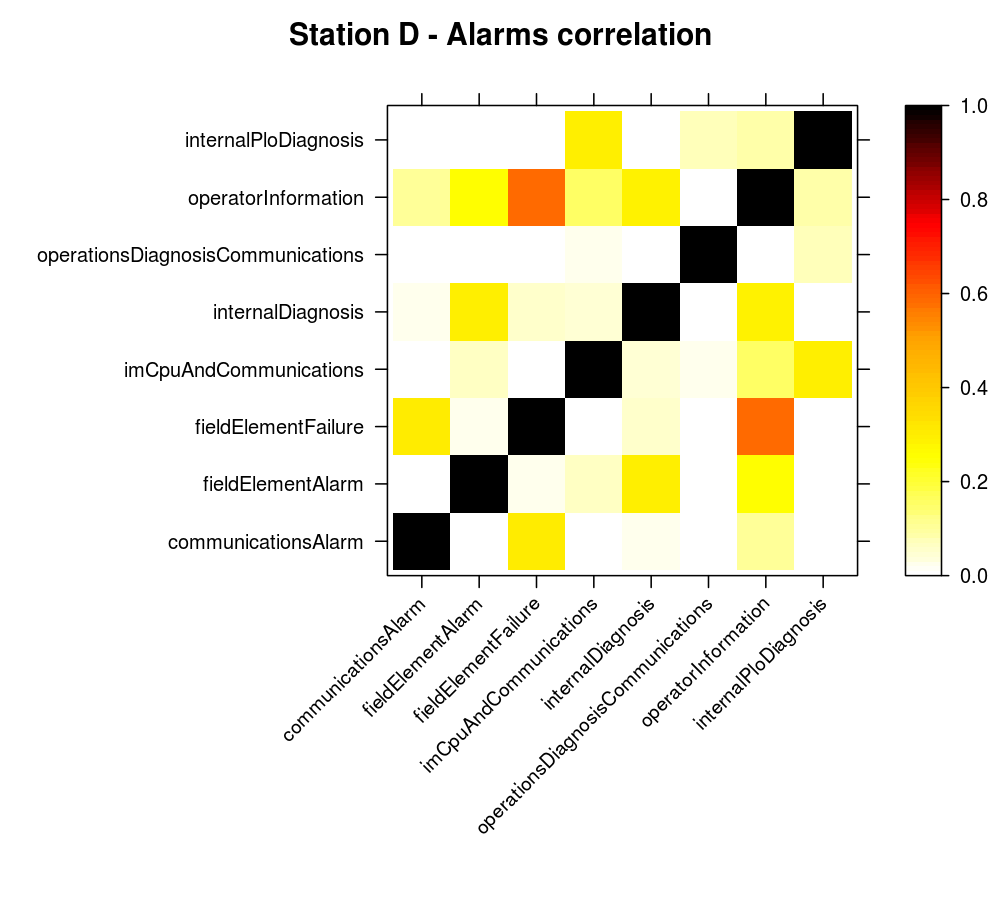
\includegraphics[width=\textwidth]{./img/sevilla_corr.png}
 \caption{Daily correlation for Station D} \label{fig:sevilla_corr}
\end{figure}

\clearpage

At first sight, we can affirm that these relations are different even in stations A, B and D, which we found to have similar diagnosis systems. This indicates that, even with similar diagnosis systems, the systems conforming both lines are different. This is indeed confirmed by Thales' engineers, as Stations A and B control high speed lines, while Station D corresponds to a commuter line.

Furthermore, we can see strong correlations in Station D (Field element failure and operator information) and Station C (Communications alarms and processing error alarms). As we don't have deep information of the nature of these categories, we can't affirm that this high correlation is due to any causal relation. However, we observe that both these cases show high correlation for the type of alarm which is more frequent in each station, so uneven distribution of alarms might be the cause of this apparent relation between alarms.

From this analysis we can conclude the significant differences in alarm relations between stations, confirming our first thoughts of impossibility of reducing the problem by generalising and merging data from different stations. Further analysis using specific alarm identifiers instead of categories will be needed to obtain relevant results.

\clearpage

\section{Working methods}
\label{sec:methods} For the development of this project, we have found a vast amount of useful tools and software which will provide an invaluable help in the different processes of our work. The main tool used will be the \emph{R} language\cite{ihaka1996r}, a very powerful tool commonly used for handling large amounts of data in an efficient way, and for which a vast amount of tools are available for our needs. R, and the IDE we are using, \emph{RStudio}\cite{racine2012rstudio} are open source software and available at no cost.

Due to licensing and compatibility issues, we are not able to use \emph{Microsoft SQL Server} databases to handle data. This is highly inconvenient as the data provided by Thales is in form of MS SQL backup files, which we needed to migrate to a compatible system of our choice: \emph{MySQL}. Given the tabular nature of the data, another solution based on plain text files would not be recommendable - although possible to handle with R - at least at the earliest stages until we analyse all the information and reduce the number of variables to export. In order to perform these migration tasks, a \emph{Windows} platform with \emph{Microsoft SQL Server Express} was required. Migration was successfully possible after slight modification of indexes and field definitions to fix compatibility issues. Once in MySQL format, we can query our data from RStudio without being limited to any kind of platform type or operative system, and will indeed perform further stages of the project under \emph{Unix} platforms.

Among all the available algorithms which can be useful for our project, we have chosen the \emph{cSPADE} algorithm\cite{zaki2001spade} as our starting point. It provides the most straight-away solution for the kind of problem we are approaching, as it considers temporal characteristics and allows us to set time constraints very easily. Other algorithms will be studied and applied at convenience, in order to complement cSPADE and find weak points which we could improve.

\begin{table}
\begin{tabularx}{\textwidth}{|X|l|X|}
\hline \headcell{Goal} & \headcell{Priority} & \headcell{Method} \\ 
\hline
\hline Perform a preliminary statistical analysis to set the project grounds & Compulsory & Statistical analysis with R \\ 
\hline Identify differences between maintenance stations & Compulsory & Statistical analysis with R \\ 
\hline Obtain rules to predict alarms using data of other alarms occurrence & Compulsory & Data Mining algorithms with R \\  
\hline Validate and evaluate rule sets. Determine confidence of predictions & Compulsory & Cross-validation and confidence analysis with R \\ 
\hline Identify rule sets which can be applied to different station types & Desirable & Inter-station cross-validation with R \\ 
\hline Obtain rules to predict events using data of system and environment variables & Optional & Data Mining algorithms with R \\ 
\hline Identify which system or environment variables are more decisive for alarm prediction & Optional & Data Mining algorithms with R \\ 
\hline 

\end{tabularx} 
\caption{Summary of project goals and methods} \label{tab:objectives_methods}
\end{table}


\section{Final comments}
The most important thing before starting any other step, is to completely understand the context and scenario of our project. We do not need to fully know and understand the details on the procedures of railway maintenance, as the nature of the machinery performed reparations is not of significant relevance for the achievement of the defined objectives. In any case where we would need better understanding of system functioning - such as for identifying causal relations between failure events - we would need assistance from expert employees directly related with maintenance.

At this point, we have already treated all received data in order to be able to freely handle it without restrictions from any desired system. Required conversions have been performed and all data is already prepared to be loaded and used in R scripts.

We have also defined the learning objectives for the project, and set a ground to achieve them from an \emph{Knowledge Discovery in Databases} approach. Furthermore, we have made a first insight into \emph{Data Mining} techniques and performed a first analysis on their adequacy for our project.

In the next stage of Trainmining, we will need to make a deeper insight into the provided databases. The procedures which we have already defined (time discretion and definition of observation times) will have to be performed, selecting the exact variables among all of them which are registered for each alarm.
\chapter{The Data Mining Process}
\label{chap:datamining}
\begin{chapterintro}
This chapter focuses on the most important step of our project: the \emph{Data Mining} process. This is where we will actually obtain the knowledge which will allow us to implement a predictive system.

In previous chapters we already introduced some details about Data Mining, as well as presented some of the algorithms and methods that can be used for this purpose. We will now provide a much more detailed description on the usage of the chosen method and all the steps needed for their execution. Evaluation and validation criteria and methods will be defined as well at this point. We will also describe the parameters we can adjust in this process and which will define its efficiency and the quality of the results, as well as the problems faced when choosing them and alternative methods to obtain better results.
\end{chapterintro}
\section{Data Mining and Knowledge Discovery}
In previous stages of our project we have performed preliminary analysis on our data (mostly statistical) as well as the necessary preprocessing to apply different learning techniques in the following stages. Once we have completed these tasks, it is now time to perform the techniques from which the actual knowledge will be obtained.

This step, usually refered to as \emph{Data Mining} is the most important in the whole \emph{knowledge discovery} procedure. Although data analysis and preprocessing do have a big impact on the quality of the results we will be able to achieve in the end, the choice of an appropriate data mining algorithm is essential for the whole procedure to work.

In order to find the most adequate techniques for knowledge discovery in our project, we presented in chapter~\ref{chap:enabling_technologies} a survey on some of the available techniques. Due to the vast amount of already existing implementations available for each of the different data mining categories, we won't have to make an implementation from scratch but adapt one of the already existing implementations to the characteristics of our problem by setting the necessary constraints.

\section{Acquisition of association rules}
\label{sec:rule_model}
As we mentioned previously, the most appropriate way to address our problem is the construction of a model based on association rules. This approach consists on building association predictive rules using frequent secuences in our available data as a base.

First of all we must therefore obtain all potential sequential information (patterns) from our database, as mentioned. These sequences will be of the form $\{A, B\} \longrightarrow \{C, D\} \longrightarrow \{E, F\}$ and will serve as a basis to build candidate \emph{association rules}. This step is explained with further details on section~\ref{sec:mining_sequences}.

Using the frequent sequences obtained from the first step, we can build \emph{candidate association rules}. Candidate association rules are of the form $\{A, B\} \xrightarrow{T} \{C\}$. It is important to notice that in these rules we are putting additional temporal information (a distance of T between terms). This temporal information is not implicit in our previous temporal sequences, but can be inferred from the conditions used on the process to obtain them. This will be explained in detail in section~\ref{sec:assoc_rules}.

Finally, we must check which of these \emph{candidate association rules} are actually good predictive rules, and obtain a precise measure of \emph{how good} they are. Specifically, we will measure the \emph{certainty} (precision) of the predictions made by using these rules and the \emph{amount of events} (recall) they are able to predict. This step will be explained in detail in section~\ref{sec:validation_evaluation}.

The whole procedure can be summarized in the following steps:
\begin{enumerate}
\item Mining frequent sequences
\item Building candidate association rules
\item Validate the obtained rules
\end{enumerate}

These steps will be further described in the following sections.

\subsection{Obtaining frequent sequences}
\label{sec:mining_sequences}
The first step for our chosen approach is to find frequent sequences in our datasets. Frequent sequences will be good candidates from which we can be able to obtain association rules -- if there is an unknown causal relation between two events, they will appear together considerably often. Several algorithms have been developed in the past in order to approach this task of finding frequent sequences. Some examples are the \emph{GSB}\cite{zaki2001spade} algorithm and the \emph{SPADE}\cite{zaki2001spade} algorithm, being the later an alternative to the first with better performance and results.

The procedure of finding frequent sequences in a dataset mainly consists on an iterative analysis of all the possible combinations of elements of the database in sequences. For example, the GSB algorithm can be roughly described as follows:

\begin{enumerate}
\item All the possible items (events) of the database are counted. These elements can be seen as sequences of length 1, which will be subsequences of any other larger sequence.
\item All the possible length 2 candidates are generated, as combination of length 1 sequences
\item The database is scanned to calculate the support of generated length 2 candidates
\item Length 3 candidates are generated as addition of length 1 sequences to length 2 sequences whose support is higher than a given minimum
\item The process is repeated till no candidates have high enough support
\end{enumerate}

In other words, the candidates are created in a tree fashion, by adding length 1 sequences (possible terms) to elements in a level. If a branch reaches the minimum required support value, it stops growing, as adding more terms to the sequence will make it more specific and necessarily less frequent.

The support of a sequence is calculated as the number of times it happens in our dataset. The support is usually expressed as a percentage of the whole amount of sequences in the database, but it is important to note that this parameter is not related in any way with the confidence or precision of any prediction we might do with the given pattern. A deeper approach on this issue will be described later in this document.

More information on GSB and SPADE algorithms can be found in \cite{zaki2001spade, zhao2003sequential, srikant1996mining}. Although It is not our priority now to study these algorithms in depth, previous work shows a better performance for SPADE than for GSB, and therefore it will be our algorithm of choice for our work. Furthermore, SPADE implementations are conveniently available in R\cite{ihaka1996r} libraries, which will allow us to easily execute the algorithm on our datasets.

\subsubsection{Defining constraints}
One of the main problems we find when we look for frequent sequences in our database, is that not any sequence -- although frequent -- is useful for our purposes. In the end our goal is to make predictions, for which obtaining these frequent patterns is useful. However, our project context -- and sometimes common sense -- may put additional conditions on \emph{which} kind of predictions are useful; and therefore, \emph{which} kind of patterns we must look for.

For instance, due to the characteristics of our systems, it might not be possible to perform maintenance tasks in short periods of time. Sequences showing us that \emph{A} always breaks within one hour after \emph{B} breaking might not be useful even if we can obtain a very high certainty of that prediction. If we need to buy new pieces to fix B, and those pieces are usually delivered in terms of weeks, knowing that \emph{B} will break one hour before it breaks would not give us any advantage over waiting for it to break and notice without any prediction.

In other words: we need to define temporal constraints in order to obtain sensible predictions\cite{zaki2000cspade}. These constraints are the following:

\begin{description}
\item[Observation time.] We must define for how long we want to take events into account. For example, our predictions for tomorrow will be most likely be made taking into account today's events, as those from last week are less likely to be related with those happening in the short future.
\item[Minimum gap.] This is the minimum amount of time in which we want to predict events. For instance, a gap of 0 would result in predictions for events simultaneous to the observed ones, while a gap of 1 would result in predictions only for the following observation periods.
\item[Maximum gap.] The maximum amount of observations between events in our sequences. By fixing it to the same amount as minimum gap we can obtain sequences with a fixed gap between events.
\item[Maximum window.] This is the maximum temporal length for our sequences. It is important to stress that this is the length of the whole sequence, while the gap is the separation of events within a sequence.
\end{description}

Given these constraints, we have sequences with the following structure:

$$\{A, B\} \xrightarrow{T_1} \{C, D\} \xrightarrow{T_2} \{E, F\}$$

Where $mingap \leq \{T_1, T_2\} \leq maxgap$, and $T_1+T_2 \leq maxwin$. It is important to remark that these temporal conditions are not inherent to the sequences obtained by the SPADE algorithm. As we mentioned in section \ref{sec:mining_sequences}, sequences are built from all the possible combination of events, and then their support is calculated by checking how many times that sequence appears in the database. It is in support calculation where these constraints apply, but the candidate sequences do not contain any temporal information at all. We will only know that their values will be comprised within the ranges we have defined.

In this sequence we have three terms with two events each. In order to build association rules, it is very convenient to limit the number of terms to two -- a single \emph{antecedent} and a single \emph{consequent}. Furthermore, it is very convenient to limit the number of events to one, in order to make individual predictions for each of the events (which may have, for example, different certainties). 

Therefore, the previous example sequence can be divided in three subsequences of two terms:
$$\{A, B\} \longrightarrow \{C, D\}$$
$$\{C, D\} \longrightarrow \{E, F\}$$
$$\{A, B\} \longrightarrow \{E, F\}$$

And, furthermore, each of them can be divided into two subsequences with only one item in the last term:

$$\{A, B\} \longrightarrow \{C\}$$
$$\{A, B\} \longrightarrow \{D\}$$
$$\{C, D\} \longrightarrow \{E\}$$
$$\{C, D\} \longrightarrow \{F\}$$
$$\{A, B\} \longrightarrow \{E\}$$
$$\{A, B\} \longrightarrow \{F\}$$

These sequences are in fact subsequences of the original one, and therefore their individual support values will always be higher than the support original one. This means that these subsequences will already have been obtained as frequent sequences by the SPADE algorithm, without the need of performing division on the longer sequences. As a result, we can simply drop the sequences whose length or complexity is inconvenient for our purposes, as their shorter subsequences will be already found by SPADE.

This results in additional length constraints:
\begin{description}
\item[Maximum terms.] The maximum number of terms in the sequence. In our previous example, we should have set it to \emph{2}.
\item[Maximum items per term.] This condition defines the maximum amount of items in each of the terms of the sequence. This is \emph{not exactly} what we wanted to achieve with our second division of sequences, as we only want to apply this condition to the last term and not to all of them. In our previous example, we would have to set this limit to 1 but only for the last term of the sequence.
\end{description}

Both these groups of constraints must be applied within the process of the algorithms which will obtain the frequent sequences from our database. The length constraints will limit the construction of \emph{candidate sequences} and the temporal constraints will put conditions to the calculation of \emph{sequence support}. Its implementation must therefore be made into the sequence mining algorithms.

An extended version of the SPADE algorithm has been developed to include some of these constraints which were not contemplated by the original SPADE implementation. The \emph{cSPADE} algorithm\cite{zaki2000cspade,wu2010sequential} provides an implementation taking into account all these mentioned conditions. It is available as an R implementation under the library \emph{arulessequences}\cite{hahsler2011arules}. The only constraint which we are not directly able to define as a cSPADE condition is the maximum number of items in the last term of the sequence, as the condition imposable as a cSPADE parameter is a maximum number of items for \emph{all} the terms. This will have to be addressed at the time of building the association rules, as we will see in section \ref{sec:assoc_rules}.

\subsection{Building candidate association rules} 
\label{sec:assoc_rules}
The next step in our knowledge discovery process is the construction of potential rules which could be applied to the prediction of events in our system. As we have mentioned several times, a rule is a sentence of the form ${A} \xrightarrow{T} {B} [p]$, where \emph{A} is the antecedent (maybe containing several events), B is the consequent (also maybe containing several events), \emph{T} is the time period between \emph{A} and \emph{B}, and \emph{p} is the probability of this rule being true.

In order to transform our already available set of frequent sequences into rules of said form, first we must build all the candidate rules which can result from the obtained sequences. As we mentioned in section \ref{sec:mining_sequences}, \emph{cSPADE} allows us to define certain constraints in order to obtain suitable sequences to build rules afterwards. Said constraints are:

\begin{itemize}
\item Maximum of two terms per sequence. We will set this to \emph{2}, as mentioned in section \ref{sec:mining_sequences}.
\item Gap between terms (\emph{T}) comprised between mingap and maxgap. As we are working only with two terms, this defines also the maximum length for the sequence.
\item Maximum number of events in a term. We cannot however define independent limits for each of the terms, as we would like
\end{itemize}

It is important to remember that our data is, at this point, divided into \emph{observations}. Observations are discrete periods of time in which we group events. When we speak of \emph{gaps} and \emph{temporal lengths} we are always speaking in terms of observations, and therefore the real temporal conditions will depend on the length we defined for our observations.

In order to achieve an exact value for T, instead of having to work with ranges, we will set the maximum gap and the minimum gap to the same value. If we want, however, to find rules for a larger range of T values, we can iteratively repeat this process increasing its value. This will provide us with independent rules for each value of T, which will allow us to evaluate and validate them independently, resulting in better results. 

We will therefore have sequences of the following form:

$$\{A, B\} \longrightarrow \{C, D\}$$

As we mentioned before, we will divide these into subsequences with a single item on the last term of the sequence. More exactly, we will disregard sequences that do not comply this condition, as their valid subsequences will also have been detected by cSPADE. The result will be the following:

$$\{A, B\} \longrightarrow \{C\}$$
$$\{A, B\} \longrightarrow \{D\}$$

In order to convert these sequences into rules, we simply need to assign them a \emph{T} value and an associate probability \emph{p}. The definition of \emph{T} is quite immediate, as we have defined exactly the gap we want to have in sequences by setting maxgap and mingap to the same value. The probability \emph{p} will be calculated in the next stage, and will be the factor deciding whether \emph{candidate rules} become actual \emph{prediction rules} or not (as well as a very important performance factor and predictive information).

At this step, we must therefore only gather those sequences which fall into our conditions and give them a temporal value \emph{T}. Simple as that, the process mainly consists on subsetting tasks performed with simple R scripts, which will give us the following:

$$\{A, B\} \xrightarrow{T} \{C\}$$
$$\{A, B\} \xrightarrow{T} \{D\}$$

At this point we have transformed the initial frequent sequences into candidate association rules. The next step is to check which of these candidate rules are actually useful for predictive purposes. This leads to the last steps in the construction of this model: \emph{evaluation and validation}.


\subsection{Evaluation and validation}
\label{sec:validation_evaluation}

Once we have obtained a set of candidate rules, we must evaluate them to discern which of them are good enough to make it into the final predictive rule set. For this, we must perform two final tasks: defining evaluation criteria and applying a validation method.

\subsubsection{Evaluation criteria}
In order to evaluate and validate our rules, we must first define the evaluation criteria. This is, what will make a rule better or worse than others.

The main goal in our project is the implementation of tools which will give us a prediction using current events as its input. As a first thought, we can immediately think of evaluating our predictions by how true they actually are. We can measure the \emph{accuracy} of a prediction rule system easily by checking how often it becomes true and how often it does not. This is an important factor to take into account, but is however not the only significant indicator of the quality of the system. In a limit case in which we only attained a trivial but highly accurate rule which gives valid but trivial predictions all the times, we would have an accuracy of 100\%, while the overall quality of the system would be none. We must actually check not only the accuracy of our predictions, but also their relevance against the whole situation.

Therefore, we will need two different evaluation parameters: one related to the accuracy of our predictions, and other related to the fraction of events we are able to predict\cite{torgo2003data}. In first place, we will define \emph{precision} as the fraction of our predictions which are accurate. In the case of evaluating a rule against a test set, $P_{accurate}$ would be the number of times when both the antecedent and consequent of the given rule have happened within the stipulated time window; while $P_{total}$ would be the number of times when the antecedent of the given rule has happened, whether the consequent has or has not happened. Prediction can be as well calculated for a whole rule set, or for any kind of system which gives a predicted event based on other input events.

\begin{equation}
Prec_i = \dfrac{ P_{i, accurate}}{ P_{i, total} }
\end{equation}

On the other hand, we will define \emph{recall} as the relation between events which have successfully been predicted by our system ($E_{predicted}$) and the total number of events ($E_{total}$). 

\begin{equation}
Rec_i = \dfrac{ E_{i, predicted}}{ E_{i, total} }
\end{equation}

Notice that the number of events which have been predicted ($E_{predicted}$) is, in fact, the number of accurate predictions as calculated in the definition of \emph{precision}, ($P_{accurate}$)

In other words, precision is the ratio between accurate predictions and the total number of predictions; while recall is the ratio between accurate predictions and the total number of events.

It is important to notice that in our context, an event can't be \emph{wrongly} predicted. Our prediction can be either true or false, but if we make a prediction of the type $\{A, B\} \longrightarrow \{C\}$ and instead we observe that $\{A, B\} \longrightarrow \{D\}$; it does not mean in any way that we predicted C instead of D, but that our prediction of C was false and we did not predict D. As a result, some other tools generally used to complement values of precision and recall (such as \emph{confusion matrices}) cannot be applied in our case.

Taking a further step, we can merge both indicators in a single one, obtaining a single indicator for a much easier evaluation. Precision and recall are often merged in the called \emph{F-measure}, defined as:
\begin{equation}
F = \dfrac{(\beta^{2}+1) \cdot Prec \cdot Rec}{\beta^{2} \cdot Prec+Rec}
\end{equation}
where $\beta\in [0,1]$ balances the importance between recall and precision.

In order to obtain high precision values, we must usually compromise recall and vice versa. Very precise rules will usually require strict conditions, which will reflect situations so specific that there is few probabilities of failure. On the other hand, these strict conditions will only happen a quite limited amount of times, resulting in a low recall value. If we want however to obtain high recall values (predicting a high percentage of the total events) we will be using very general rules, into which most of the situations can fall. More general rules will however result in less precise predictions, as the possibilities that they reflect are much higher, both for situations in which the prediction would be true and those in which the prediction would be false.

In our project, we must look for rules with high precision values, whichever their recall is. In most scenarios, it will be better to count on precise predictions -- having the certainty of our predictions being good -- than to predict more events but at the compromise of their credibility.

Therefore, we will use precision value as the main evaluation parameter.

\subsubsection{Validation method}
Once we have defined the evaluation parameters we must calculate the performance of our candidate rules in order to assign precision values to each of them. Precision information is also part of the information we want to give in our predictions, so a proper calculation is of essential importance.

However, if we do this on the same data we have used to obtain this knowledge (our \emph{learning set}) we will obviously obtain extremely good results, as we have already learnt all the patterns happening on that exact data. If we had an ideal, infinite data set with \emph{all} the possible situations that can ever happen in our scenario, we could have learnt absolutely every possible prediction to be made on the system and no future event could be \emph{unexpected} to our new prediction abilities. However, in real systems this is not the case, and it is very likely that patterns and characteristics of the systems vary along time. 

Additionally, training our system over a single large set of data can lead to \emph{overfitting}. This happens when our predictive knowledge becomes extremely accurate for the set we have been training on, but performs poorly on any other set of events not contained on our learning set. It is important to avoid overfitting by performing learning procedures in a way that not our whole amount of data available is used at the same time. In this direction, the usage of very large data sets for learning procedures can be very inconvenient. In one hand we might be learning patterns which are exclusive to the specific period we are studying (for instance, we may be trying to obtain knowledge from logs from a specific year which we intend to use for forthcoming years), and when we validate this information, we will obtain unrealistic good performance measures.

In order to make a proper validation of the obtained knowledge, we must separate our data in different sets. One of them will be the \emph{learning set} -- over which we will work to obtain our predictive knowledge -- and the other will be used as a \emph{testing set} -- on which we will test our predictive abilities. This way we will obtain a better validation of our predictive knowledge, as the characteristics of the testing set were not taken into account on the learning process, as  would happen for any future set of events.

In order to address this problem, one of the most used methods is the \textit{k}-fold cross-validation (\textit{k}-fold CV) method. This method consists on dividing the whole data set in \textit{k} subsets of equal sizes, using \textit{k-1} of them as the learning set and the \textit{k}th one as the testing set. Performance results are stored for those specific learning and testing sets and the whole process is repeated a total of \textit{k} times, until all the possible learning sets/testing sets combinations are obtained.

With this process, we obtain a total of \textit{k} performance testing results for our model. The important point is that all of them have been tested on sets which were not used for their construction. The overall performance measure is obtained as the arithmetic mean of all the individual performance results.

In some cases, we can even randomize the division of the data into subsets, obtaining different subsets for each process of \textit{k}-fold CV we perform. In our case, however, we are limited in this direction by the nature of our data, as it is very important to preserve sequential information of our data. Our subsets must therefore be conformed of contiguous observations, and cannot be randomized between different temporal subsamples.

A commonly used value for \textit{k} is 10. As in our case we will generally work with data sets comprising about a year of historic data, this division will provide learning sets of about 9 months and testing sets of about 1 month, which reasonable when validating predictions in terms of days.

\section{Adjusting search parameters}
\label{sec:search_parameters}
The results of the whole mentioned process will be determined by its execution parameters. In sections~\ref{sec:mining_sequences} and~\ref{sec:assoc_rules} we already explained all the possible adjustments we can make in both steps and how they would affect to obtained results. 

For this kind of data mining algorithms, what most influences the quality of results is search depth. In other words, they will be determined by how \emph{deep} in our data we are willing (or \emph{able}) to search in order to find our desired information. The deeper we search, the better results we can expect, at the cost of higher need of resources.

In our problem, depth comes defined by two parameters: number of terms and minimum sequence support.

The \emph{maximum number of terms} is simply how long we want our sequence candidates to be. The more items we add to a sequence, the more specific that situation will be, from which we can expect to obtain more precise information. However, the more specific a situation is, the less likely it will be to be extrapolated to usual situations. In terms of computation, the length of the candidates exponentially rises the complexity of the problem and the number of resources needed, and therefore a reasonable limit is to be put on this parameter.

The \emph{minimum support} defines the number of times a sequence needs to have happened to be considered \emph{frequent}. This parameter has already been mentioned in the explanation of the chosen algorithm in section~\ref{sec:mining_sequences}. A lower minimum support value will offer a higher number of candidates, and therefore a higher number of association rules. However, this parameter drastically affects the computational costs needed to execute the algorithm.

As we mentioned in section~\ref{sec:mining_sequences}, candidates are built in a tree fashion, with branches growing larger and larger till the minimum support is reached. Both parameters define when branches of the trees stop growing: once the maximum number of terms has been reached, or once the support is not enough for the sequences to be considered frequent. A compromise must therefore be found between both parameters, in order to be able to search as deep as possible.

\emph{Minimum support} does not have any effect on the obtained rules. Reducing it will generate a higher number of candidates and rules, but their quality or characteristics won't have any relation with this parameter. The \emph{maximum number of terms}, however, does affect them. Longer rules will usually be much less adequate than shorter ones. If we could predict \emph{everything} just by knowing one of the events which have happened today, it would be much better than having to wait till ten of them happen in order to be able to predict anything. However, it is very likely that we can make good predictions counting on very little information, so longer rules could be expected to have higher performance values.

The decision criteria is then clear for the minimum support: we want to set this to the minimum value which can be handled by our computation capabilities. In terms of number of terms, however, increasing depth will provide \emph{more} results, some of which will however be too long as to be actually useful.

\subsection{Determining optimal values for search parameters}
In order to fix the maximum number of terms in sequences, we have executed the whole process in a smaller sample of data with a considerably high maximum value of terms. Setting this value to \emph{10}, we could analyse results for sequences of different lengths. It is important to note that although we could expect longer sequences always to be more precise, they will also be much less frequent, so we will much faster reach the minimum support limit obtaining less candidates and probably worse rules. For this analysis, the selected minimum support was of \emph{0.1}.

The results are shown in table~\ref{tab:maxprecision_test}.

\begin{table}
\begin{center}
\begin{tabular}{|c|c|c|}
\hline \headcell{Antecedent length} & \headcell{Maximum precision} \\ 
\hline 
1 & 0.43 \\ 
\hline 
2 & 0.51 \\ 
\hline 
3 & 0.76 \\ 
\hline 
4 & 0.83 \\ 
\hline 
5 & 0.83 \\ 
\hline
6 & 0.32 \\ 
\hline 
7 & --- \\ 
\hline 

\end{tabular} 
\caption{Possible maximum length parameters. Test execution} \label{tab:maxprecision_test}
\end{center}
\end{table}

In this test run, no candidates were found with lengths of over 7 terms and support higher than 0.1. We also see that for values of 6, precision starts to decay as fewer candidates are found, with which not very good rules could be generated. We will therefore generally choose a value of 5 as the maximum size of candidates, and up to 7 in cases in which the minimum support can be significantly reduced (smaller or divided data sets).

The choice for minimum support is obvious. We will choose the minimum value our computation capabilities can handle. As this is difficult to determine beforehand, we will follow a trial and error method. Starting from values of 0.01, we will iteratively increase it when computation fails to finish in a period of 24 hours.

The details of the server used for these operations can be seen in table~\ref{tab:server}.

\begin{table}
\begin{center}
\begin{tabular}{|c|c|c|}
\hline \headcell{Item} & \headcell{Details} \\ 
\hline 
Processor &  Intel(R) Core(TM) i7 CPU 950 @ 3.07GHz \\ 
\hline 
Number of cores & 8 \\ 
\hline 
Memory & 12 GB \\ 
\hline 
OS & Ubuntu 11.10 Server \\ 
\hline 

\end{tabular} 
\caption{Server details} \label{tab:server}
\end{center}
\end{table}

\clearpage
\section{Data clustering for complexity reduction}
\label{sec:dataclustering}
As seen in section~\ref{sec:search_parameters}, computation capabilities can significantly limit our search depth, forcing us to use lower depth values and therefore compromising the quality of the results. In order to be able to use higher depth values, we can either increase our computation capabilities or look for a way to decrease the complexity of the problem.

Increasing capabilities is not a feasible option. Our server is actually running a top end configuration on which there is few possible room for improvement. Although memory or CPU speed could be increased, these improvements would be so small that our limitations would be reduced ever so slightly. The only option is therefore trying to divide our problem into different smaller problems.

For this purpose, we will divide our data into several clusters, depending on the type of alarms. Thales' database already counts on alarm categorisation, dividing them into different types depending on which station we are working with. Alternatively, we can try to create clusters based on different criteria. It is important to note that in order to be able to use the obtained information in the whole system afterwards, cluster intersection must be zero for whichever criteria we follow. In other words, a specific type of event can only happen in one of the clusters, so that a relation found being true in one of them cannot be false in other situation.

We will try two different approaches for this purpose: division by already defined alarm types, and clustering by type of physical elements.

\subsection{Using already defined alarm types}
\label{sec:using_event_type}
The most immediate possible division is to divide our datasets into many containing only one type of alarm. This complies with the \emph{empty intersection} condition, as every different possible event can only fall into one of the categories. The most important limitation is that using this method, we won't be able to find rules relating alarms of different types. It is also important to note that for each of the stations, the event-type distribution is not uniform, and therefore different improvement in possible search depth will be achieved for each of the generated clusters.

First of all, we will make an insight on the size of the resulting clusters for each of the stations. These sizes can be seen in figures \ref{fig:clusters_alb} to \ref{fig:clusters_sev}. At first glance we observe not only a very unequal distribution of alarms into these clusters, but also that some of them are unadequately small. For clusters whose size is less than tens of thousands alarms we can expect significantly worse results. Although such a small size allows us to use very high values for search depth, the amount of data available can be too small for any information to be extracted.

The rule of thumb used to determine possible search depths for each of the clusters depending on their size is shown in table~\ref{tab:thumbrule}. This rule is the result of a trial and error procedure, and does not guarrantee the ability for computation as the real performance depends on the individual characteristics of the datasets.

As a result, this clustering method allows us to perform much deeper searches at least in some of the groups. Taking the whole databases at once forced us to set a significantly low search depth value, which resulted either on very low quality results (few rules with low precision) or on the complete unability to perform the process with the available computation capabilities.

\begin{figure}[hbtp]
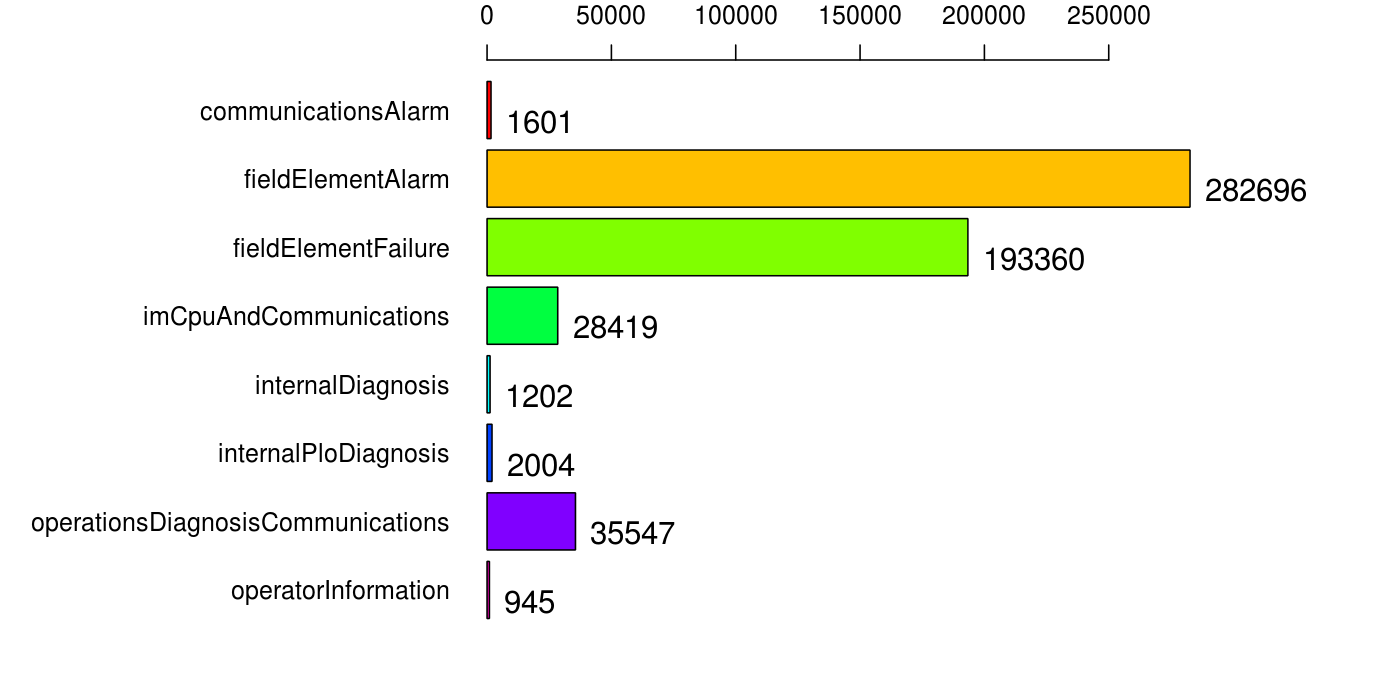
\includegraphics[width=\textwidth]{img/clusters_alb.png}
\caption{Clusters and their size for Station A} \label{fig:clusters_alb}
\end{figure}

\begin{figure}[hbtp]
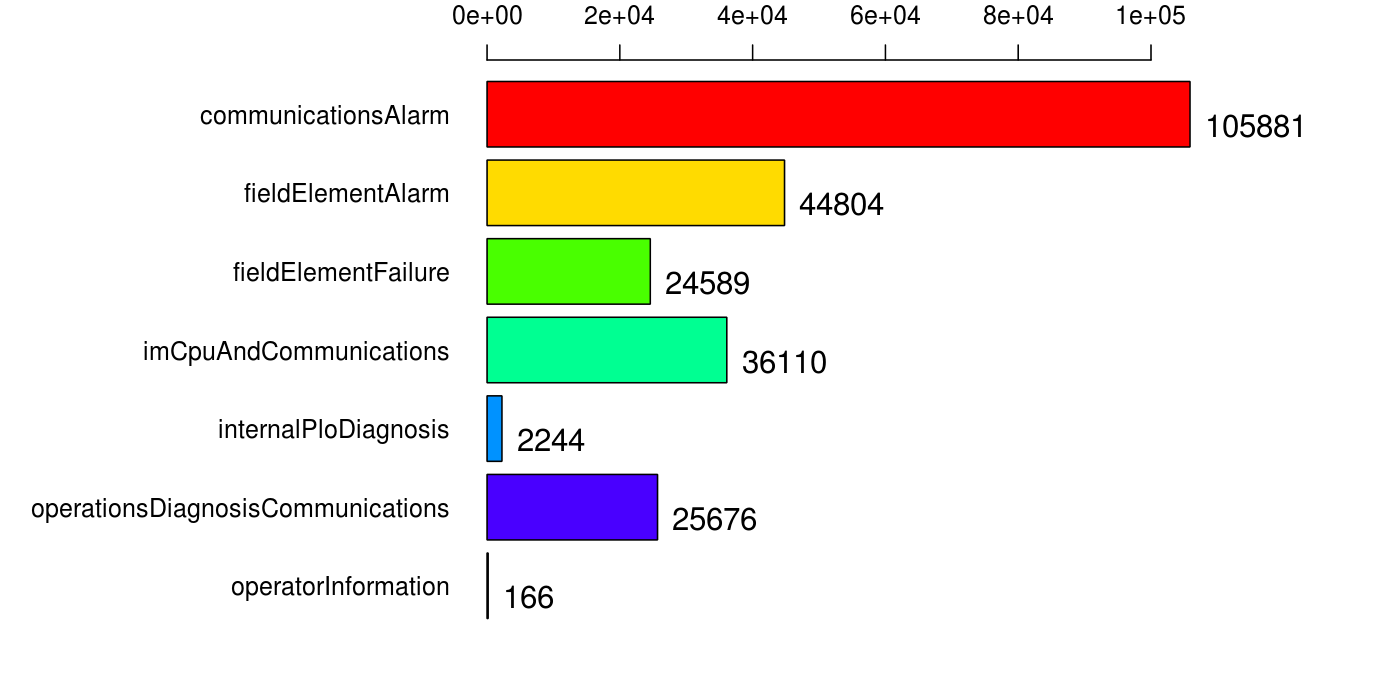
\includegraphics[width=\textwidth]{img/clusters_ant.png}
\caption{Clusters and their size for Station B} \label{fig:clusters_ant}
\end{figure}

\begin{figure}[hbtp]
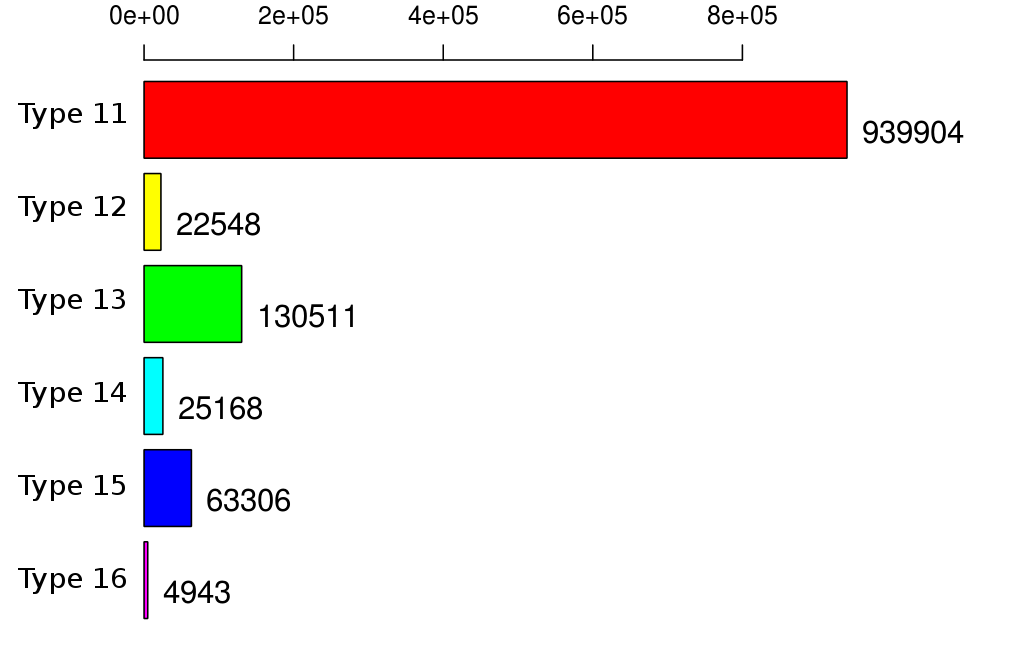
\includegraphics[width=\textwidth]{img/clusters_seg.png}
\caption{Clusters and their size for Station C} \label{fig:clusters_seg}
\end{figure}

\begin{figure}[hbtp]
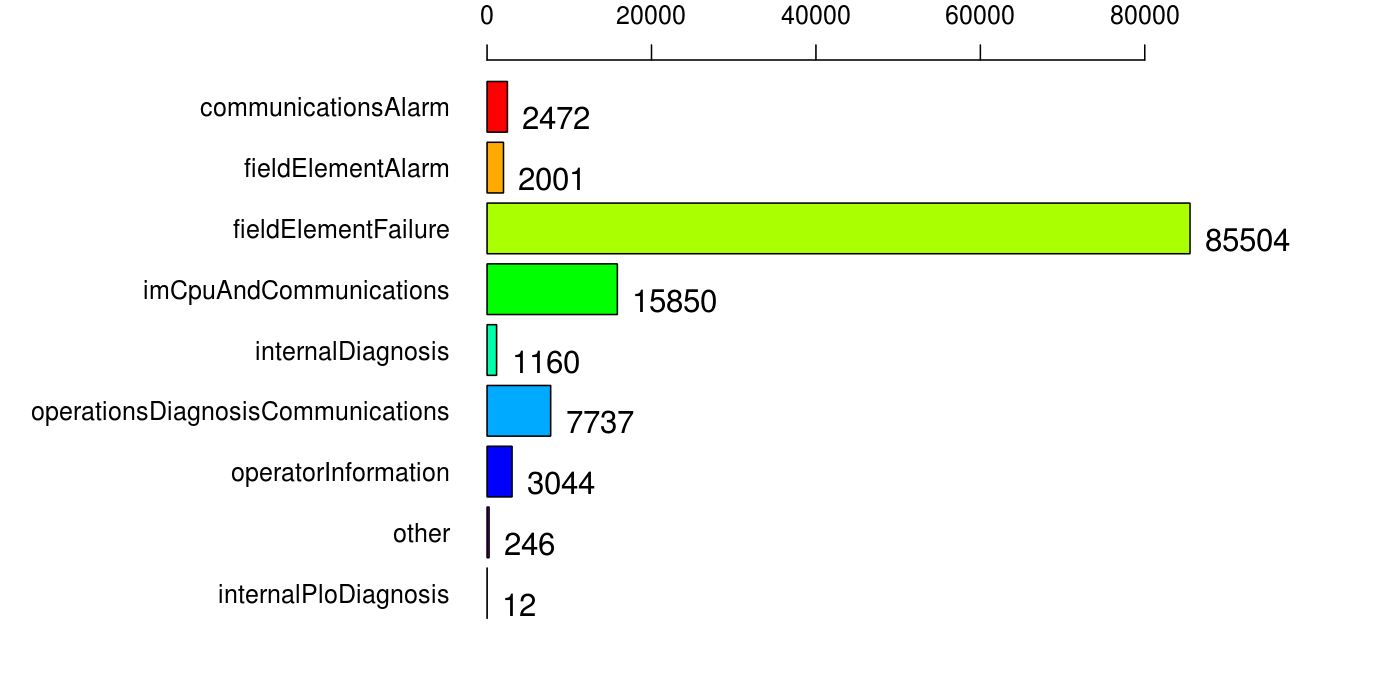
\includegraphics[width=\textwidth]{img/clusters_sev.png}
\caption{Clusters and their size for Station D} \label{fig:clusters_sev}
\end{figure}


\begin{table}
\begin{center}
\begin{tabular}{|c|c|c|}
\hline \headcell{Cluster size} & \headcell{Maximum number of antecedents} & \headcell{Minimum support} \\ 
\hline 
$<$ 10.000 & 7 & 0.01 \\ 
\hline 
10.000 - 50.000 & 5 & 0.1 \\ 
\hline 
50.000 - 100.000 & 5 & 0.2 \\ 
\hline 
$>$100.000 & 5 & 0.3 \\ 
\hline 

\end{tabular} 
\caption{Search depth parameters for different cluster sizes} \label{tab:thumbrule}
\end{center}
\end{table}

\subsection{Grouping similar physical elements}
\label{sec:group_elements}
As a second method, we will try and group alarms by the element which raises them. For our \emph{empty intersection} rule to be followed, we will need to make groups which gather \emph{all} the elements which can raise the same type of alarms. Unfortunately, information on the physical elements which raise the alarms is not directly tabulated and available in the provided databases. The corresponding element is instead included as part of the message shown to the operator, sometimes along with other parameters, and therefore this classification cannot be directly made.

In order to achieve this, we will check, for all the different possible events, their associated \emph{ADDITIONAL\_INFOS} field, which depends on (but not corresponds to) the raising elements. By looking for similar naming patterns on said field, we might be able to find a way to perform this desired way of clustering. Most of the groups did not follow evident patterns at first sight, but after analysing all their relations with different alarms, we were able to come with several clusters. The created groups for Station B can be seen in table~\ref{tab:custom_clusters}. For example, \emph{ADDITIONAL\_INFOS} fields of the form E1, E2, E3... always were found in lights-related alarms, same as for the form R1, R2, R3... and therefore all the events falling into these conditions will be clustered into the \emph{lights} cluster.

These groups do not follow any official categorisation made by Thales' engineers. Although an index of physical elements existed and was available, its relation with the alarms in the database was not direct. Furthermore, what we want to achieve is groups of elements which are likely to raise similar elements (and to follow similar patterns in their occurence) and therefore we do not need these groups to be actually made by exact classification of the types of elements.

Comparison of results with and without this kind of clustering can be seen in figure~\ref{fig:group_vs_nogroup}. The number of high-precision rules significantly increases by using this kind of clustering. Further comments on the results can be found in chapter~\ref{chap:results}.

This process, however, must be made manually looking for different patterns and elements which seem to raise the same type of events. Therefore, it is a very time consuming process and its not suitable for being applied systematically to all datasets. The provided data corresponds to the Station B, for which we have performed the procedure in order to evaluate its possible benefits. In order for this to be suitable for general application, additional info should be provided in datasets which could allow faster automatic grouping.

\begin{table}
\begin{center}
\begin{tabular}{|c|c|c|}
\hline \headcell{ADDITIONAL\_INFOS pattern} & \headcell{Cluster} \\ 
\hline 
A00, A01, A02... & Switches \\ 
\hline 
10, 11, 12... 140 & Lights \\ 
\hline 
E1, E2, E3, E4 ... & Lights \\ 
\hline 
S1/1, S1/2 ... & Lights \\ 
\hline 
R1, R2, R3 ... & Lights \\ 
\hline 
M1, M2, M3 ... & Lights \\ 
\hline 
A|XX|XX & Communications \\ 
\hline 
B|XX|XX & Communications \\ 
\hline 
IM|XX|XX & Communications \\ 
\hline 
EC|XX|XX & Communications \\ 
\hline
EN-A, EN-B, EN-M & Electric network and power supply \\ 
\hline   
ALI\_XXX & Electric network and power supply \\ 
\hline   
Alimentacion XXX & Electric network and power supply \\ 
\hline   
V1, V2 ... & Rail tracks \\ 
\hline   

\end{tabular} 
\caption{Clusters found for different patterns in ADDITIONAL\_INFOS field} \label{tab:custom_clusters}
\end{center}
\end{table}

\begin{figure}[hbtp]
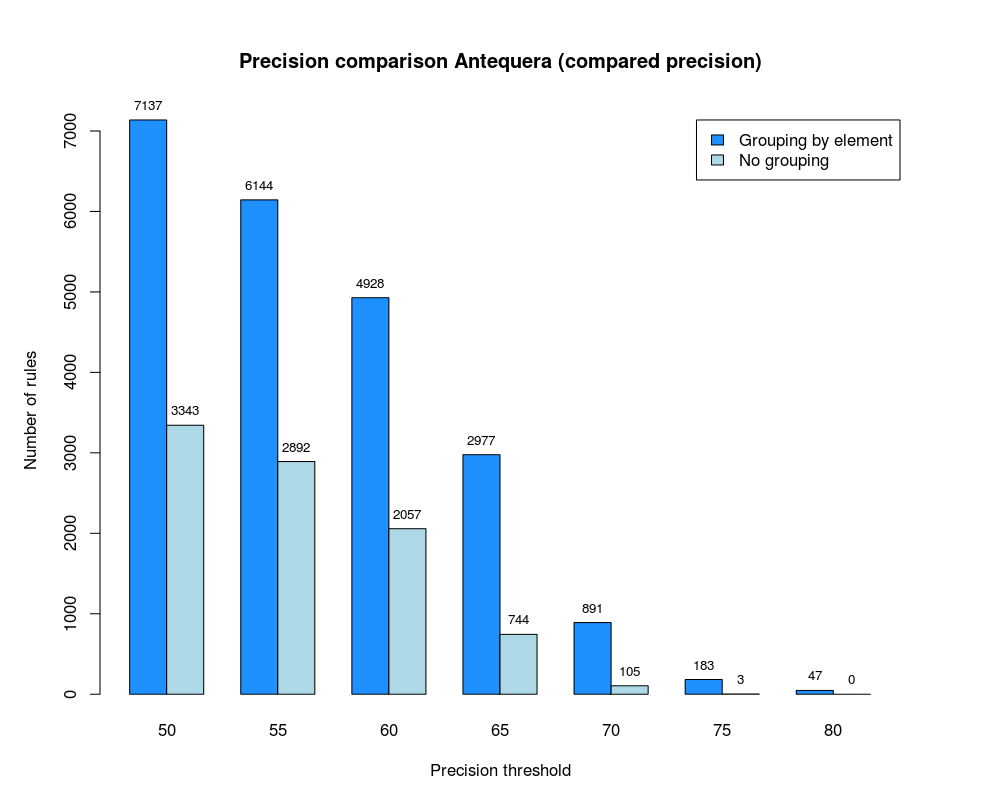
\includegraphics[width=\textwidth]{img/group_vs_nogroup.png}
\caption{Number of rules by precision before and after grouping by similar elements} \label{fig:group_vs_nogroup}
\end{figure}


\chapter{Prototype Implementation}
\label{chap:prototype}

\section{Module description}
\label{sec:module_description}
In this section we will provide a general description of the implemented prototype. This prototype allows the usage of already existing association rules, which have been already obtained as the result of a \emph{Data Mining}\cite{torgo2003data}\cite{han2006data} procedure. These rules do not offer any functionality by themselves, as a system is needed to check whether their conditions are fulfilled and therefore a prediction can be made.

Rules are simply textual information in the form of "When A and B happen together, C has 80\% chances of happening". This information would be useful for an operator who might be manually checking events and would be able to expect C after seeing A and B. However, real systems usually have a much larger set of possible events, and many more events happening during each observation, and therefore an automated system is needed to perform these operations.

We call such a system a \emph{Rule engine}\cite{liang2009openrulebench}. A rule engine is simply a system which evaluates input conditions and fires the rules which comply with these conditions, outputting the result of said rules. In our case, the system will take as input a set of current events, and output a list of predictions along with their probabilities.

The implementation of a rule engine is not a trivial matter, and requires a significant amount of work to achieve optimal results in terms of computation requirements and complexity. Therefore, we will count on one of the already existing solutions which suits our needs perfectly and in a very optimised way: the JBoss Drools Expert library\cite{browne2009jboss}. This library is freely available as a java module and counts on several interoperability options, which makes it perfect for the usage in our project. The only requirement this imposes is the need of translating our rules to a Drools-compatible format, a matter which will be addressed later on this document.

\subsection{Parameters and interfaces}
\label{sec:parameters_and_interfaces}
Depending on our needs for each situation, our system can obtain predictions for several periods of time, different types of systems and different input lengths. Specifically, we count on rules for four different stations of different characteristics (Stations A, B, C and D) and for three different time windows (one day, two days and seven days). Each of these prediction modes needs a different type of input and needs to use a different set of rules. This distinction has therefore been made at the time of generating the rules, and now those rules need to be loaded accordingly to the kind of prediction we want to obtain.

In other words, said parameters (station type and time window) fixes the set of rules to be used and the length of the input to be provided. This association also works in the other direction: by using an specific rule set and an specific input, we are already defining the execution parameters. Therefore, both the station type and prediction time window are irrelevant for the correct function of our predictive module. It is responsibility of the operator or executing system to select the appropriate rule set and provide an appropriate input. This allows new execution options to be added or updated at any time, without the need of modifying the module in any way. If we generate a new set of rules expecting a whole month of input and which will generate a month of predictions, we just need to load it and know what it is generating. Also, if we generate rules for a new type of maintenance station we just need to load them on the module and provide an input according to that new type of station.

The architecture of the module is very simple. It counts on an Engine class which streamlines the whole procedure, relying on three model classes to provide Alarm and prediction representations. A class diagram can be seen in figure~\ref{fig:prototypeArchitecture}

\begin{figure}[hbtp]
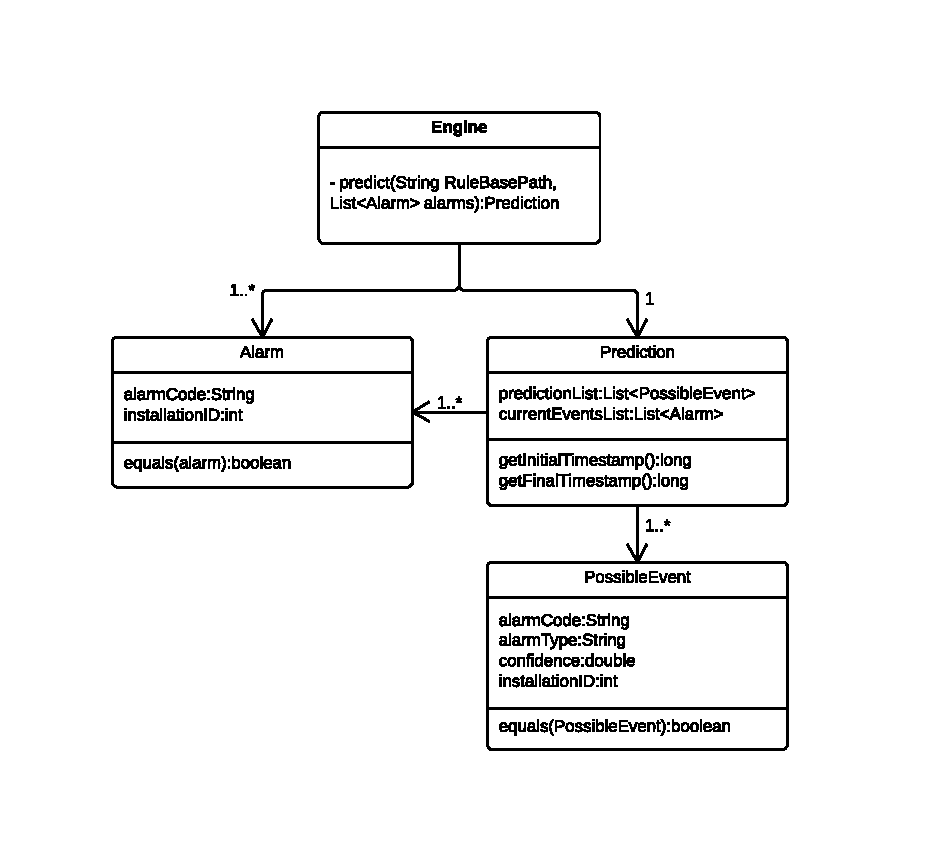
\includegraphics[width=\textwidth]{img/prototypeArchitecture.pdf}
\caption{Class diagram for the implemented module} \label{fig:prototypeArchitecture}
\end{figure}

\subsection{Input selection and execution}
As described in section~\ref{sec:parameters_and_interfaces}, our module takes a list of Alarm objects and outputs a Prediction object containing a list of PossibleEvent objects. We have also seen that it is important to provide an input which adequates to the conditions imposed by the selected rule set (or viceversa), which simply means that we must provide a list containing an observation time whose length adequates to that expected by the rule set.

Furthermore, as seen in figure~\ref{fig:prototypeArchitecture}, Alarms are described not only by their alarm code, but also by the installation in which they have been raised. It is important to have into account that alarms are only related to others happening in the same installation, and therefore we only need inputs to contain sets which are complete in terms of installation id. In other words, we could call the inference engine with separated inputs containing each the alarms which have been raised by each of the installations. However, as the rule sets are the same for all of the installations under the same maintenance station, it is more efficient to make this distinction during execution instead of having to call the engine and load the rules several times.

\subsection{The rule engine}
In section~\ref{sec:module_description} we introduced the concept of \emph{the rule engine}, the core of our module in which most of the heavy processing happens. Amongst all the available solutions, we selected the \emph{Drools Expert}\cite{browne2009jboss} platform, as it is the most advanced solution available for Java environments, and therefore an easy integration can be made with the rest of the maintenance station software.

\emph{Drools Expert} relies on \emph{Drools rule files}, which are plain text files containing our rules coded with an special syntax. Furthermore, it provides several ways of managing and even changing these rules, as interfaces for business users or other tools to easily generate these files based on workflow diagrams or other sources. However, as the knowledge on which our rules are based is obtained from a different source (a fully independent Data Mining process) we won't make use of these posibilities and will just have to consider the output format for our rules, to make it directly compatible with Drools' syntax. In section~\ref{sec:description_of_rule_sets} we will provide further description of these rule sets, as well as their generation and conversion processes.

Our module encapsulates and streamlines the execution of Drools Expert and their preparation process. The details of this configuration are of little relevance, and can be summarized as \emph{choosing a rule set} and \emph{provide a valid input}. Our module will then simply evaluate all the rules and then provide an output with a prediction for the next period, as we described in section~\ref{sec:parameters_and_interfaces}. The cornerstone of all this process is therefore the rule set. As we will describe in section~\ref{sec:description_of_rule_sets}, it is of essential importance to carefully build these in order to obtain a proper function of the rule engine. In the end, the rules are actually part of the code of our module, on which reiles most of its functionality.

A sequence diagram of the module's function can be seen in figure~\ref{fig:prototypeSequence}

\begin{figure}[hbtp]
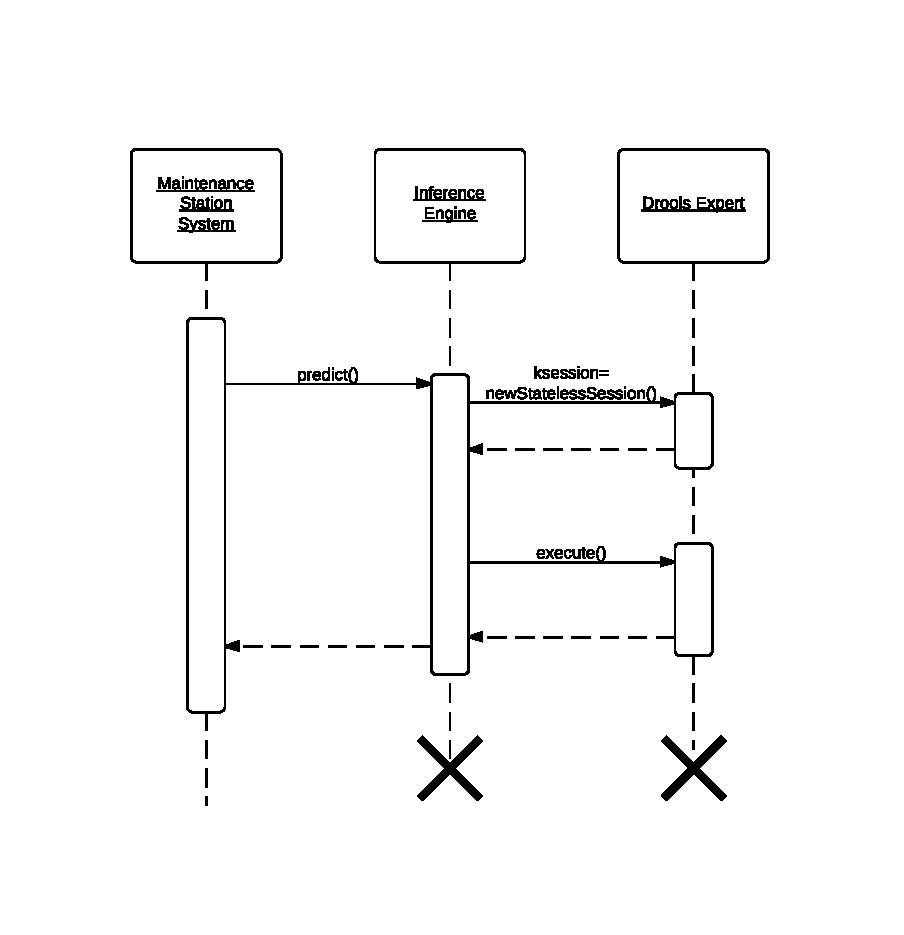
\includegraphics[width=\textwidth]{img/prototypeSequence.pdf}
\caption{Sequence diagram for the implemented module} \label{fig:prototypeSequence}
\end{figure}

\section{Description of rule sets}
\label{sec:description_of_rule_sets}
In this section we are going to describe the most important part of our prediction module: the rule sets. A rule set is simply a plain text file containing the necessary information for a rule to be evaluated and fired in the adequate circumstances. A rule can be simply seen as a piece of information stating that "When \emph{A} and \emph{B} happen, \emph{C} will happen with a certainty of 80\%", but there is actually a few more compexity added for the proper functioning of our system.

First of all, as we mentioned in section~\ref{sec:parameters_and_interfaces}, we have to take into account that events have to happen in the same installation for alarms to be raised. In other words, the rule above would be actually needed to be stated as follows:

\emph{"When A happens, and B happens in the same installation as A, C will happen in the same installation with a certainty of 80\%"}

Also, although it is not necessary for the basic function of our module, we will also return the type of alarm we are predicting in the output. The type of alarm can be directly inferred from the alarm code itself, but as we are working with hardcoded rulesets which only need to be generated once, it is much more efficient to associate the alarm type with each rule than having to perform a search every time an event is predicted. This does not affect how or module works at all, but our rule will actually look more like:

\emph{"When A happens, and B happens in the same installation as A, C (Which is an event of type 1) will happen in the same installation with a certainty of 80\%"}

This information can be useful to provide an overview of the kind of systems which are more prone to fail in a short future, and probably assign resources to groups instead of actual specific events for organisational convenience.

It is important to note that we are not mentioning at all time periods either for the observation (events A and B) or the expectation (event C). As we mentioned in section~\ref{sec:parameters_and_interfaces}, those parameters are implicit to the whole set of rules. For example, we \emph{know} we are talking of an observation of one day and a prediction for one day in the future because we are loading the ruleset whose rules work with that time windows. This is much more convenient as reduces the complexity of the rules avoiding having to handle additional parameters, but needs that the calling process takes into account these parameters by itself.

The same applies for the type of station we are working with. Even though the stations we are working with are quite different from each other, we do not specify in the rules where do we expect those events to hapen. Or we don't specify that \emph{explicitly}, because again, each rule set works exclusively for one specific station.

There is also a third parameter which we can directly affect simply by selecting an specific rule set: confidence. Instead of having to filter rules by their confidence when setting a threshold, it is much more efficient and convenient to load only those rules which provide predicitons with a confidence higher than a given threshold. As we mentioned, rulesets are plain text files which contain all the rules to be loaded, so by simply removing those with low confidence, we can perform this filtering in a very efficient way.

It is up to the maintenance operator to decide upon these thresholds. In order to be on the safe side, we usually set a threshold of 50\% (which is, predictions which are more likely to be right than wrong), but for an operator it might be more convenient to disregard maybe even predictions whose confidence are lower than 70\% or 80\%. By directly removing those rules from the rule sets, the additional computation needed to evaluate them is eliminated, and therefore the execution would be much more efficient.

The specific list of sets which have been generated and provided can be seen in table~\ref{tab:ruleset_list}.

\begin{table}
\begin{center}
\begin{tabular}{|c|c|c|c|c|}
\hline \headcell{Rule set} & \headcell{Station} & \headcell{Observation} & \headcell{Prediction} & \headcell{Min. Confidence} \\ 
\hline 
albacete1d\_70.drl & Station A & 1 day & next day & 70\% \\ 
\hline  
albacete7d\_70.drl & Station A & 7 days & next 7 days & 70\% \\ 
\hline 
antequera1d\_70.drl & Station B & 1 day & next day & 70\% \\ 
\hline 
segovia1d\_70.drl & Station C & 1 day & next day & 70\% \\ 
\hline
segovia2d\_70.drl & Station C & 2 days & next 2 days & 70\% \\  
\hline 
segovia7d\_70.drl & Station C & 7 days & next 7 days & 70\% \\  
\hline 
sevilla1d\_70.drl & Station D & 1 day & next day & 70\% \\ 
\hline
albacete1d\_50.drl & Station A & 1 day & next day & 50\% \\ 
\hline 
albacete7d\_50.drl & Station A & 7 days & next 7 days & 50\% \\ 
\hline 
antequera1d\_50.drl & Station B & 1 day & next day & 50\% \\ 
\hline 
segovia1d\_50.drl & Station C & 1 day & next day & 50\% \\ 
\hline
segovia2d\_50.drl & Station C & 2 days & next 2 days & 50\% \\  
\hline 
segovia7d\_50.drl & Station C & 7 days & next 7 days & 50\% \\  
\hline 
sevilla1d\_50.drl & Station D & 1 day & next day & 50\% \\ 
\hline
albacete1d\_all.drl & Station A & 1 day & next day & -- \\ 
\hline  
albacete7d\_all.drl & Station A & 7 days & next 7 days & -- \\ 
\hline 
antequera1d\_all.drl & Station B & 1 day & next day & -- \\ 
\hline 
segovia1d\_all.drl & Station C & 1 day & next day & -- \\ 
\hline
segovia2d\_all.drl & Station C & 2 days & next 2 days & -- \\  
\hline 
segovia7d\_all.drl & Station C & 7 days & next 7 days & -- \\  
\hline 
sevilla1d\_all.drl & Station D & 1 day & next day & -- \\ 
\hline

\end{tabular} 
\caption{Generated rule sets} \label{tab:ruleset_list}
\end{center}
\end{table}

\subsection{Generation of rule sets}
\label{sec:generation_of_rule_sets}

We have mentioned in section~\ref{sec:module_description} that our rules are obtained through a \emph{Data Mining process}, and later translated into the Drools syntax. In this section we are going to give an overview of the whole process.

Everything starts with a database backup provided by Thales' engineers which contains a large amount of event logs in all the stations we are going to study. That database is transformed into a working set, a process which involves several processes such as variable reduction, data normalisation and format conversion. This data is loaded into an R\cite{ihaka1996r, torgo2003data} environment in which the core data mining procedure is performed: the rule discovery process. This step forms the core of the whole procedure, and requires a considerable amount of resources and time.

This generates a raw list of association rules, in the format of R data frames. At this point we can already perform some filtering to separate the useful rules from those with very low confidence values. However, as those rules can also be useful for future research or to be manually analysed by maintenance operators, so far we have decided to save the whole amount of generated rules whichever their precision was.

A last process is performed in which we convert the raw R data frames\cite{ihaka1996r} containing the rules into the Drools syntax. At this point we also generate several subsets with different confidence thresholds, as mentioned in section~\ref{sec:description_of_rule_sets}. This step is fully automated with Python\cite{sanner1999python} scripts. An example of both formats will be shown in section~\ref{sec:structure_of_rules_and_sets}.

A diagram of the whole process can be seen in figure~\ref{fig:prototypeGenProcess}.

\begin{figure}[hbtp]
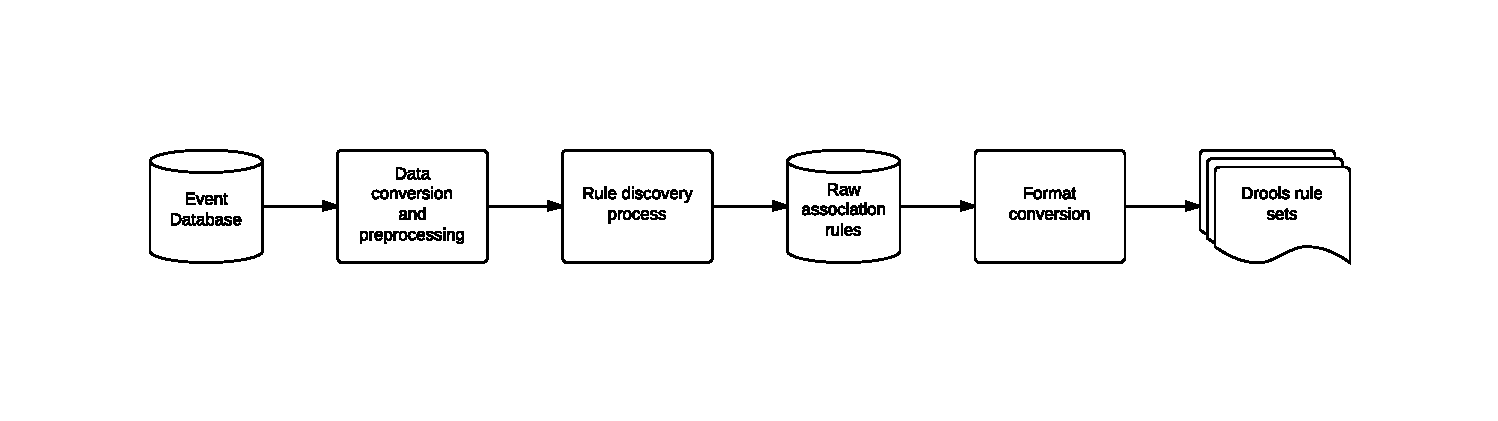
\includegraphics[width=\textwidth]{img/prototypeGenProcess.pdf}
\caption{The whole rule generation process} \label{fig:prototypeGenProcess}
\end{figure}

\subsection{Structure of rules and sets}
\label{sec:structure_of_rules_and_sets}
In this section we will now analyse the actual structure of our rules and their conversion to the Drools syntax. We will take the following rule as an illustrating example:

\begin{framed}
\begin{lstlisting}[style=mono]
"<{
	saml.status.energy_net1_not_present
	saml.status.energy_net2_not_present
	saml.status.energy_48V_battery_nok
	saml.status.energy_SAI_PT_nok
},{
	saml.status.energy_SAI_ST_nok
}>",
0.83833333,
0.089034423
\end{lstlisting}
\end{framed}

That is the appearance of a prediction rule in the format of R data frame. Lines 2, 3 and 4 are the antecedents, line 6 is the predicted event and rule 8 is the precision of the rule. The last number on line 9 is the recall of the rule, an evaluation value which is of no use at this moment.

The same rule in Drools syntax would looks as follows:

\begin{framed}
\begin{lstlisting}[style=mono]
rule "rule0"
    when 
        Alarm(iid : installationID, alarmCode 
        		== "saml.status.energy_net1_not_present");
        Alarm(installationID == iid, alarmCode 
        		== "saml.status.energy_net2_not_present");
        Alarm(installationID == iid, alarmCode 
        		== "saml.status.energy_48V_battery_nok");
        Alarm(installationID == iid, alarmCode 
        		== "saml.status.energy_SAI_PT_nok");
    then 
        PossibleEvent p = new 
        	PossibleEvent("saml.status.energy_SAI_ST_nok",
        			"fieldElementFailure",iid,0.83833333);
        resultList.add(p);
end
\end{lstlisting}
\end{framed}

We can see here the additions mentioned in section~\ref{sec:description_of_rule_sets}, regarding installation code and event type (which is hardcoded here to "filedElementFailure"). The resultList object conforms the output which will be returned by Drools to our module, containing all the generated possible events.

\section{Output visualisation}
When describing our predictive module, we haven't so far spoken on how this data is visualised or shown to maintenance operators. This is because our module does not provide a visual interface in any way to make this data user-readable. The predictive module is meant to be integrated in a much larger system which is Thales' railway maintenance station software. This will provide operators a visualization of the predictions, and can even provide means for automatic prediction handling.

However, in order to illustrate the possibilities offered by the implemented prototype, we have developed a demonstration interface. This illustrative example can be seen in figure~\ref{fig:demoExample}.

\begin{figure}[hbtp]
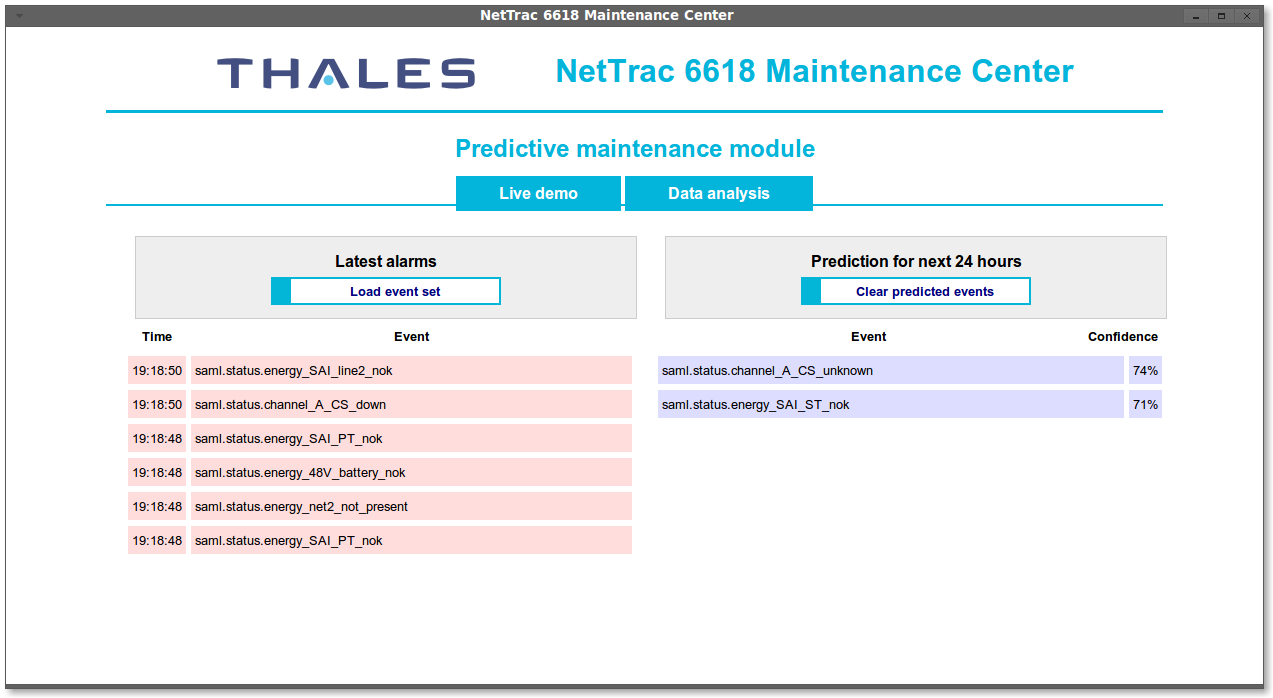
\includegraphics[width=\textwidth]{img/demoExample.png}
\caption{Example demo interface} \label{fig:demoExample}
\end{figure}

\clearpage

\section{Conclusions}
At this stage of the project, we have already developed a fully functional predictive module to be integrated within Thales' maintenance station. Furthermore, a demo interface has been provided in order to illustrate one of the multiples applications this module can offer to maintenance operators.

However, the module allows Thales' engineers to perform much more advanced tasks with these predictive information. From statistical reports including information on the predictions, to automatic processes started as response to specific predicted events, the range of possibilities is quite large.

Integration is also possible within any other kind of system, due to the implementation of the module as a Java library. Furthermore, it is even possible to build a standalone predictive system, performing predictions sobre already generated static event sets.

In general terms, the implementation of the module has been successful and completely fulfils our goals.

\clearpage

\chapter{Conclusions and Future Work}
\label{chap:conclusions}
\begin{chapterintro}
In this chapter we will gather the conclusions obtained as a result of the project, as well as possible future work that can be done for further development of this project and any other predictive tasks in general.
\end{chapterintro}
\section{Project outcomes}
The main outcome of this project is the obtention of large amounts of knowledge which can be used for predictive purpose by Thales' maintenance operators. As presented in chapter~\ref{chap:results}, we have obtained several large rulesets which can be used to predict events with high confidence values, up to 80\% in some cases.

These rulesets have been obtained for the four stations we have studied (named A, B, C and D; and located in different points across the Spanish territory). Furthermore, for each of the stations, different processes have been performed in order to obtain rules for different time periods: one day, two days and seven days. This allows maintenance operators to obtain predictions for different time periods according to what is more convenient for them. While it may be useful to predict events on a daily basis to foresee shortage times and optimise maintenance, it sometimes might be necessary to know with more days in advance in order to acquire the needed equipment or resources to solve the problems. Additionally, these rulesets also contain relations which have been found to be of low confidence, but which can still be useful for further research.

In order to obtain higher quality results, several methods have been used as described in chapter~\ref{chap:datamining}. This includes identifying changes in the data which could lead to significantly better results. Although sometimes manually and impossible to automatise for a large-scale application, this has been very useful to identify the need to better classificate alarms in terms of the systems which are raising them, which can be automatised in the future by modifying the way maintenance stations register these events.

Also, a prototype has been designed and implemented in the form of a Java library. This allows our obtained rulesets to be implemented right away within Thales' systems, which is very useful to start in-place evaluation and already allows predictive maintenance to be performed. The engine has been implemented in a modular way, so that rulesets are independent of the software itself and can therefore be added or updated anytime in a very easy way.

Furthermore, the project has allowed us to perform a deep insight into data mining techniques, and specially into the way of applying these techniques to event-based problems. The developed processes are not only useful for this specific purpose, but can also be used in any similar environment in which event-prediction can offer benefits.



\section{Achieved goals}

In chapter~\ref{chap:context_and_goals} we mentioned a list of goals for the project. The achieved goals can be summarised as follows:

\subsubsection*{Perform a preliminary statistical analysis to set the project grounds}

This goal has been achieved successfully. Its results are presented in chapter~\ref{chap:context_and_goals}

\subsubsection*{Identify differences between maintenance stations}

This goal has been achieved successfully. Through the data analysis described in chapter~\ref{chap:context_and_goals} we identified the differences between all the stations. These differences were later confirmed by Thales' engineers, who provided further information on the differences between systems in each station.

\subsubsection*{Obtain rules to predict alarms using data of other alarms occurrence}

This goal has been achieved successfully. As the main goal of the project, the results described in chapter~\ref{chap:results} refer mainly to this goal, as well as most of this document.

\subsubsection*{Validate and evaluate rule sets. Determine confidence of predictions}

This goal has been achieved successfully. The validation and evaluation processes have been a very important part of the project, and all the resultsets contain confidence information as a result of a thorough validation process, as described in chapter~\ref{chap:datamining}.

\subsubsection*{Identify rule sets which can be applied to different station types}

This goal has been achieved successfully. Due to the high differences between the studied stations, each of them has a very strictly defined set of rules which can be applied. In the case of new stations being built with similar characteristics to the existing ones, this point would need to be reevaluated.

\subsubsection*{Identify which system or environment variables are more decisive for alarm prediction}

This goal has been achieved successfully. As mentioned in chapter~\ref{chap:context_and_goals}, all database fields have been analysed in order to reduce alarm representation to the minimum. Furthermore, additional fields which could be of use to improve performance have been identified.

\section{Conclusions}
After the development of this project, we have learnt about the importance and benefits of predictive operations. We can assure than machine learning and data mining algorithms can therefore offer a very important advantage in terms of predicting behaviours and events in any kind of system.

In this specific project, one of the obtained conclusions is that it is essential to count on an appropriate data model in order to perform effective data mining. In our case, additional information about the elements which raised the alarms could have helped significantly to perform much better searches and obtain higher quality rules. Furthermore, it would also have been useful to know which alarms are more likely to be useful to identify other future events, or potential relations between them which could be known from experience by maintenance operators.

Existing algorithms for sequence mining do not usually take into account the separation between antecedents and consequents. The chosen algorithm, cSPADE, is one of the few solutions which already took this into account, which is highly recommended and benefitial in order to avoid heavy data transformation. This algorithm, however, allows for little fine-tuning, and performs searches in a way which could be simplified for specific cases like ours.

Generally, we have observed how information can be obtained from almost everywhere with the adequate techniques. Data mining is therefore something from which many different systems can benefit, from failure prediction like in ours, to process optimisation or any other kind of knowledge.
 

\section{Future work}
The project outcome can also serve as a solid base for future work and development. First of all, as mentioned in chapter~\ref{chap:datamining}, clustering is an efficient way of reducing the complexity of our problem and allows us to obtain much better results. Further improvement of these clustering methods, or their automation, could offer significant improvements over the methods developed for this project. In this direction, the obtained information can help maintenance operators to identify which information can actually be useful in terms of event classification, and allows further improvement of maintenance systems.

Also, as mentioned in chapter~\ref{chap:enabling_technologies}, there are other algorithms which can be used for this kind of problems. Although they require further adaptation or data transformation to be applicable, they could also provide good performance after the needed operations. A combination of both approaches could provide much richer datasets and better overall performance.

In this project we have performed analysis for three diferent time windows: one day, two days and seven days. A further way of improving the system usefulness would be to identify other potential good time windows and perform different analysis. Although we did not count on enough data to make monthly or yearly analysis, this is something that could be studied and developed in the future.

Finally, additional work could be done for this specific context based on different data. Instead of trying to predict events taking other events as input data, it would be possible to take other kinds of data such as system temperatures or voltage variations. At the moment of developing this project, such data cannot be automatically acquired, and therefore such analysis is not possible. However, useful information could be extracted from such data and could be useful to develop this option in the future.

\cleardoublepage
\phantomsection
\addcontentsline{toc}{chapter}{Bibliography}
\bibliographystyle{unsrt}
\bibliography{datamining}

\end{document}